\section{Dataset Construction Guidelines} \label{appendix:data_collection}

\subsection{General Principles}
\label{sec:general_principles}
Our data collection and curation follow several general principles to ensure that \textsc{QuantiPhy} is ethically sourced, physically well-defined, and suitable for quantitative evaluation.

\noindent\textbf{Copyright and ethics.}
We carefully avoid copyright and ethical issues throughout all stages of data collection and processing.
All videos, 3D assets, and simulation resources are either open-source, licensed for research use, or explicitly verified to pose no known copyright conflicts before inclusion.
When raw videos contain personally identifiable information (e.g., human faces, license plates), we apply blurring or masking to anonymize the content.

\noindent\textbf{Video selection criteria.}
To make quantitative kinematic inference well-posed and to reduce confounding factors, we enforce the following constraints on all collected videos.
\begin{itemize}[leftmargin=*]
  \item \textbf{Static camera in world coordinates.}
  The camera remains fixed in the world frame during each clip.
  This avoids entangling camera motion with object motion, which would otherwise introduce additional ambiguity and noise into the inference problem.
    \item \textbf{At least one rigid object undergoing translational motion.}
    Each video contains at least one rigid object whose dominant motion is translation.
    This requirement ensures that we can formulate well-defined kinematic inference tasks.
    Non-rigid objects and purely rotational motions are left out of the current benchmark and deferred to future work.\footnote{In this work, we adopt a relaxed definition of rigid objects: we consider an object ``rigid'' if its motion can be consistently approximated by a stable center of mass across frames. This includes some entities that may exhibit slight non-rigid deformation (e.g., a flying bird or a walking person), as long as their motion remains locally trackable and structurally coherent.}
  \item \textbf{Planar motion for \texttt{2D} tasks.}
  For \texttt{2D} instances, the target object and the reasoning target are constrained to move in a plane parallel to the image plane, i.e., the depth relative to the camera remains (approximately) constant over time.
  This assumption guarantees a consistent mapping between pixel displacement and world-space distance within each clip, making the 2D kinematic inference problem well-defined.
\end{itemize}

\noindent\textbf{Video–text record schema.}
Each annotated instance in \textsc{QuantiPhy} is represented as a structured video–text record.
Table~\ref{tab:record-schema-example} shows a representative example.

\begin{table*}[t]
\centering
\small
% \setlength{\tabcolsep}{4pt}
\renewcommand{\arraystretch}{1.1}
\begin{tabular}{l p{0.68\linewidth}}
\toprule
Property & Example value \\
\midrule
\texttt{\textbf{video\_id}} &
\texttt{simulation\_0032} \\
\texttt{\textbf{video\_source}} &
\texttt{simulation} \\
\texttt{\textbf{video\_type}} &
\texttt{A3MC} \\
\texttt{\textbf{fps}} &
\texttt{30} \\
\texttt{\textbf{inference\_type}} &
\texttt{DD} \\
\texttt{\textbf{question}} &
\texttt{What is the acceleration of the orange car at 1.0s in m/s\textsuperscript{2}?} \\
\texttt{\textbf{ground\_truth\_prior}} &
\texttt{gravity acc = 9.8 m/s\textsuperscript{2}} \\
\texttt{\textbf{depth\_info}} &
\texttt{t=1s, distance\_ball\_camera = 13.80 m;}\\[-0.2em]
&
\texttt{t=2s, distance\_ball\_camera = 13.80 m;}\\[-0.2em]
&
\texttt{t=1.5s, distance\_orange\_camera = 10.18 m;}\\[-0.2em]
&
\texttt{t=2s, distance\_orange\_camera = 10.40 m;}\\[-0.2em]
&
\texttt{t=2.5s, distance\_green\_camera = 4.32 m;}\\[-0.2em]
&
\texttt{t=3s, distance\_green\_camera = 6.91 m} \\
\texttt{\textbf{ground\_truth\_posterior}} &
\texttt{2.86} \\
\bottomrule
\end{tabular}
\caption{\textbf{Example of a single video--text record in \textsc{QuantiPhy}.}}
\label{tab:record-schema-example}
\end{table*}

Each record contains the following fields:
\begin{enumerate}[leftmargin=*]
  \item \textbf{\texttt{video\_id}.} A unique identifier for the underlying video.
  \item \textbf{\texttt{video\_source}.} The data source from which the video was obtained (e.g., \texttt{simulation}, \texttt{lab}, or \texttt{internet}).
  \item \textbf{\texttt{video\_type}.} A four-letter code encoding the configuration of the task.
  The four characters denote, in order: (i) the type of physical prior (Size, Velocity, or Acceleration), (ii) whether the reasoning task is \texttt{2D} or \texttt{3D}, (iii) whether there is a single (\texttt{S}) or multiple (\texttt{M}) moving objects, and (iv) the background type, that is, plain (\texttt{X}), simple (\texttt{S}), or complex (\texttt{C}). More details are included in \autoref{subsec:video_type}.
  \item \textbf{\texttt{fps}.} The frame rate of the video, used to convert frame indices into time and to compute velocities/accelerations consistently.
  \item \textbf{\texttt{inference\_type}.} A two-letter code indicating whether the prior and the inference target are static or dynamic over time:
  \texttt{S} denotes a static quantity, and \texttt{D} denotes a time-dependent (dynamic) one.
  The first letter corresponds to the prior, and the second to the posterior.
  \item \textbf{\texttt{question}.} The natural-language prompt presented to the VLM.
  We ensure that each question explicitly specifies the physical unit (e.g., m, cm/s, m/s\textsuperscript{2}) and, for velocity or acceleration, clearly indicates whether the query concerns an instantaneous quantity at a given timestamp or an average quantity over an interval.
  \item \textbf{\texttt{ground\_truth\_prior}.} The physical prior provided to the model, formatted as a positive numeric value with unit (e.g., \texttt{gravity acc = 9.8 m/s\textsuperscript{2}}).
  We enforce consistent formatting to simplify parsing and downstream use.
  \item \textbf{\texttt{depth\_info}.} Depth annotations used only for 3D reasoning tasks.
  This field contains depth values (in metric units) for the prior object and, when needed, for the inference target at one or more timestamps.
  Depth information is designed so that, in principle, the depth of the inference target can be recovered from the provided entries.
  The formatting mirrors that of \textbf{\texttt{ground\_truth\_prior}}.
  \item \textbf{\texttt{ground\_truth\_posterior}.} The numeric ground-truth answer to the kinematic inference question, represented as a positive scalar without unit (the unit is part of the question text).
\end{enumerate}

\noindent\textbf{Balance and diversity.}
Finally, we design the dataset to be both balanced across task types and diverse in content.
\begin{itemize}[leftmargin=*]
  \item \textbf{Fine-grained video types.}
  Using the four-letter \textbf{\texttt{video\_type}} code, we partition all clips into 36 fine-grained categories.
  We ensure that each category contains at least four videos, so that every configuration is represented non-trivially.
  \item \textbf{Balanced core task categories.}
  We strive to keep the four core inference task categories (\texttt{2D-Static}, \texttt{2D-Dynamic}, \texttt{3D-Static}, \texttt{3D-Dynamic}) approximately balanced in terms of the number of videos and associated questions, enabling fair comparison across conditions.
  \item \textbf{Rich scenes and motion patterns.}
  We cover a broad spectrum of spatial scales and motion types.
  Scenes range from astronomical (e.g., planetary motion), to everyday macroscopic settings (e.g., traffic, sports), to microscopic phenomena (e.g., cells and bacteria).
  Motion patterns include uniform motion, accelerated and decelerated linear motion, projectile motion, pendulum-like oscillations, and centripetal motion, among others.
  This diversity is crucial for probing whether VLMs’ quantitative reasoning generalizes beyond narrow, highly stylized scenarios.
\end{itemize}

\subsection{Video Types}
\label{subsec:video_type}
\subsubsection{Video Categories Definition}
As described in the section , we assign each video a four-character code that encodes its physical prior, dimensionality, object setting, and background type.

\noindent\textbf{First character (\texttt{S} / \texttt{V} / \texttt{A}).}
The first character specifies which physical prior the video is constructed to probe. For a designated object in the scene, we use
\begin{itemize}[leftmargin=1.6em,topsep=0.2em,itemsep=0pt]
  \item \texttt{S} = size
  \item \texttt{V} = velocity
  \item \texttt{A} = acceleration
\end{itemize}
Thus, the first character takes one of $\{\texttt{S}, \texttt{V}, \texttt{A}\}$, indicating whether the ground-truth physical quantity is size, velocity, or acceleration for that object, as illustrated in \autoref{fig:SVA_scene}.

\begin{figure*}[ht!]
    \centering
    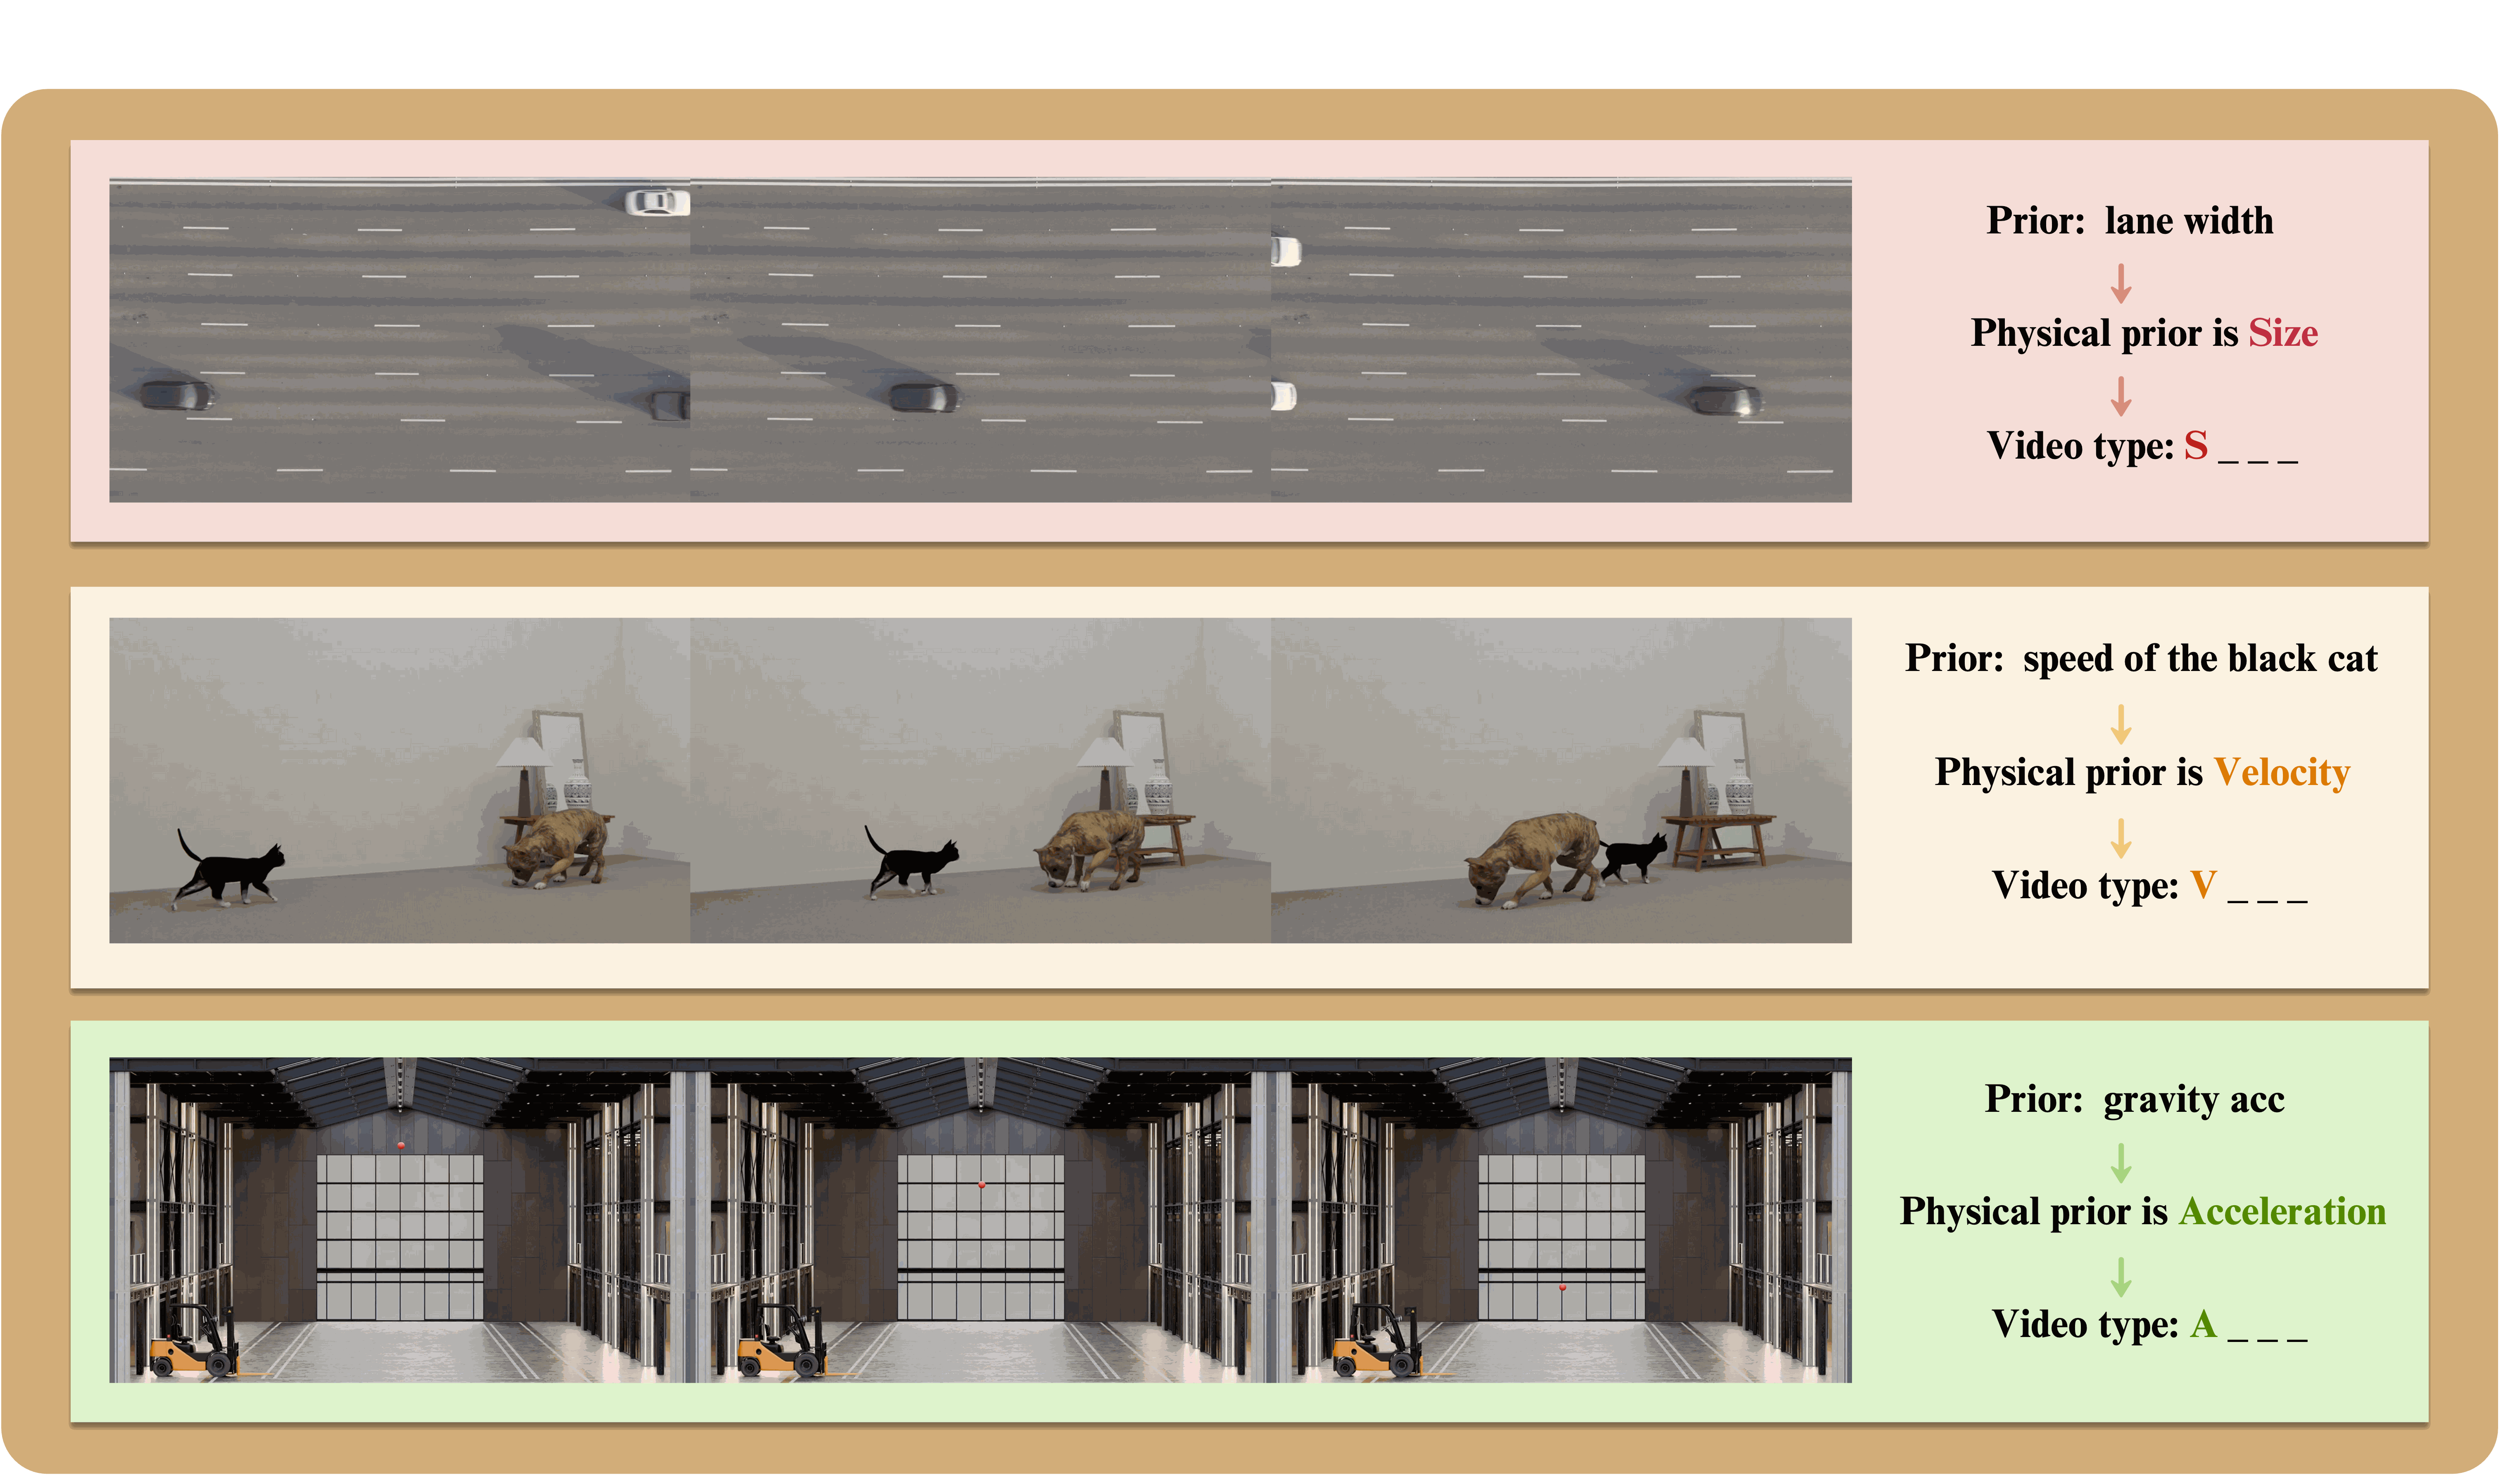
\includegraphics[width=0.99\linewidth]{sec/images/SVA.png}
    \caption{\textbf{Examples of S/V/A scene.}}
    \label{fig:SVA_scene}
\end{figure*}

\noindent\textbf{Second character (\texttt{2} / \texttt{3}).}
The second character indicates whether the video is 2-Dimensional(\texttt{2D}) or 3-Dimensional(\texttt{3D}).
\begin{itemize}[leftmargin=1.6em,topsep=0.2em,itemsep=0pt]
  \item \texttt{2D} = planar video
  \item \texttt{3D} = volumetric video
\end{itemize}
More precisely, the second character is set to \texttt{2} when, at every frame, the distances from the moving object, the ground-truth reference object, and every object referenced in the inference question to the camera are exactly equal, so they occupy a single depth layer with no relative depth or parallax among them in the rendered image, and to \texttt{3} otherwise. Video examples are shown in \autoref{fig:2/3_scene}.

\begin{figure*}[ht!]
    \centering
    \includegraphics[width=0.99\linewidth]{sec/images/2_3.png}
    \caption{\textbf{Examples of 2/3 scene.}}
    \label{fig:2/3_scene}
\end{figure*}

\noindent\textbf{Third character (\texttt{S} / \texttt{M}).}
The third character distinguishes between “single-object” and “multiple-object” settings, relative to the queried object(s) rather than the sheer number of objects visible in the scene:
\begin{itemize}[leftmargin=1.6em,topsep=0.2em,itemsep=0pt]
  \item \texttt{S} = single-object
  \item \texttt{M} = multiple-object
\end{itemize}
As shown in \autoref{fig:s/m_scene}, this label depends on how many objects the viewer needs to reason about. We use \texttt{S} (single-object) when the reasoning process only involves one object. Other objects may appear, but they only serve as background or generic distractors. We use \texttt{M} (multiple-object) when answering any of the questions requires reasoning about two or more objects, for example by comparing their sizes or speeds, or by using one object as an explicit reference for another.

\begin{figure*}[ht!]
    \centering
    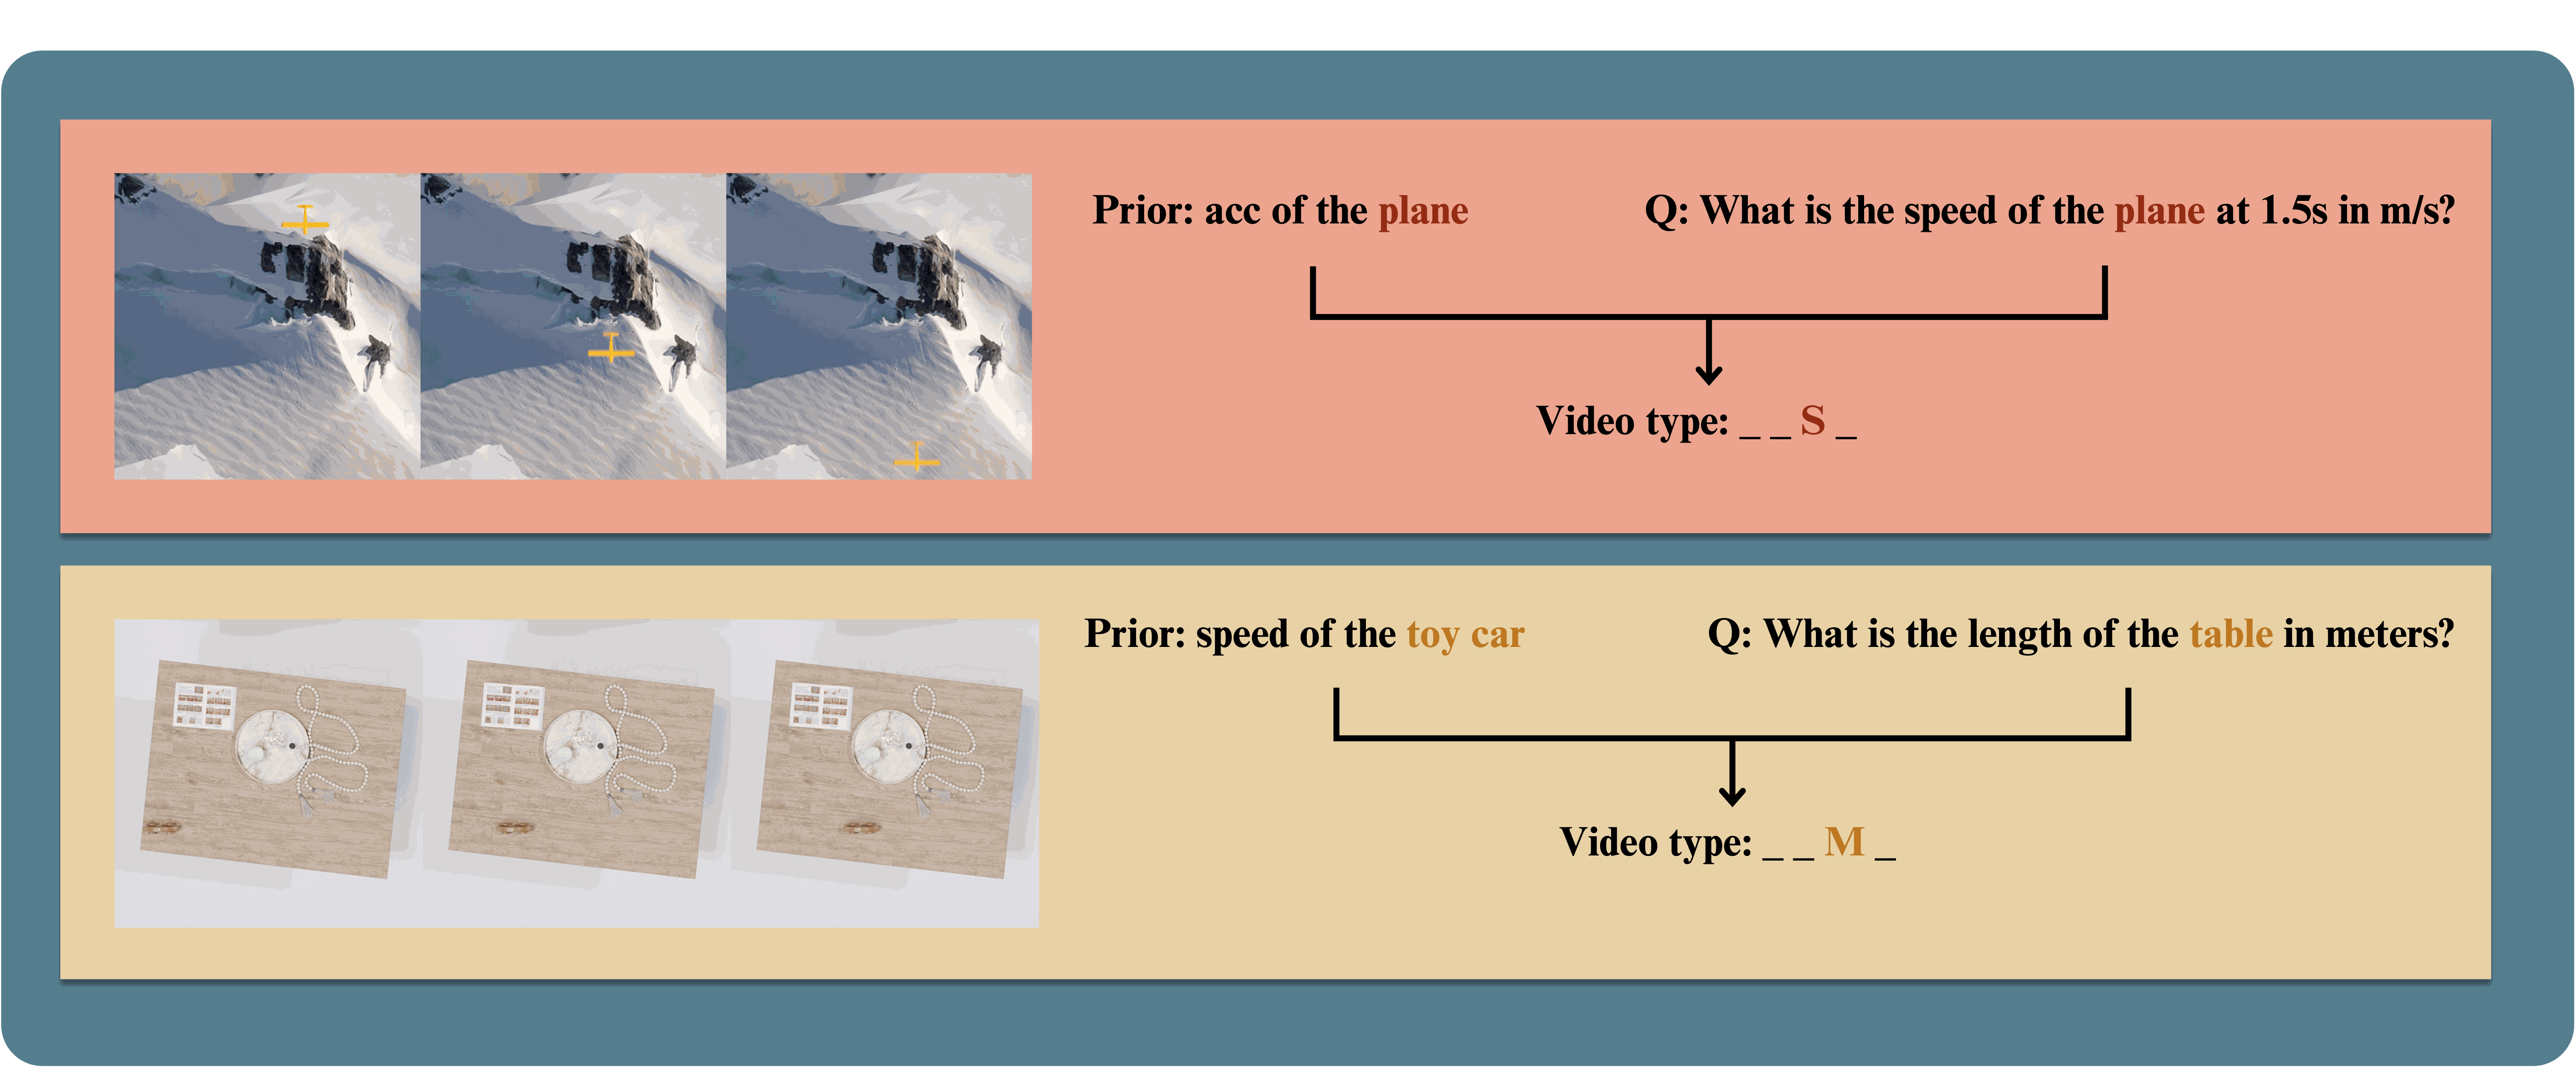
\includegraphics[width=0.99\linewidth]{sec/images/s_m.png}
    \caption{\textbf{Examples of S/M scene.}}
    \label{fig:s/m_scene}
\end{figure*}

\noindent\textbf{Fourth character (\texttt{X} / \texttt{S} / \texttt{C}).}
The fourth character's examples are illustrated in the Figure~\ref {fig:X/S/C_scene}. encodes the complexity of the background.
\begin{itemize}[leftmargin=1.6em,topsep=0.2em,itemsep=0pt]
  \item \texttt{X} = plain background, typically a single uniform RGB color with essentially no texture, clutter, or noise;
  \item \texttt{S} = simple background, which may contain mild lighting or shading variations but remains visually uncluttered;
  \item \texttt{C} = complex background, with rich textures, multiple visible objects, more intricate lighting, and substantial visual ``noise''.
\end{itemize}
The boundary between “simple” and “complex” backgrounds is somewhat subjective, but during dataset construction we deliberately separated these categories and designed scenes so that their visual difference is as clear as possible.

\begin{figure*}[ht!]
    \centering
    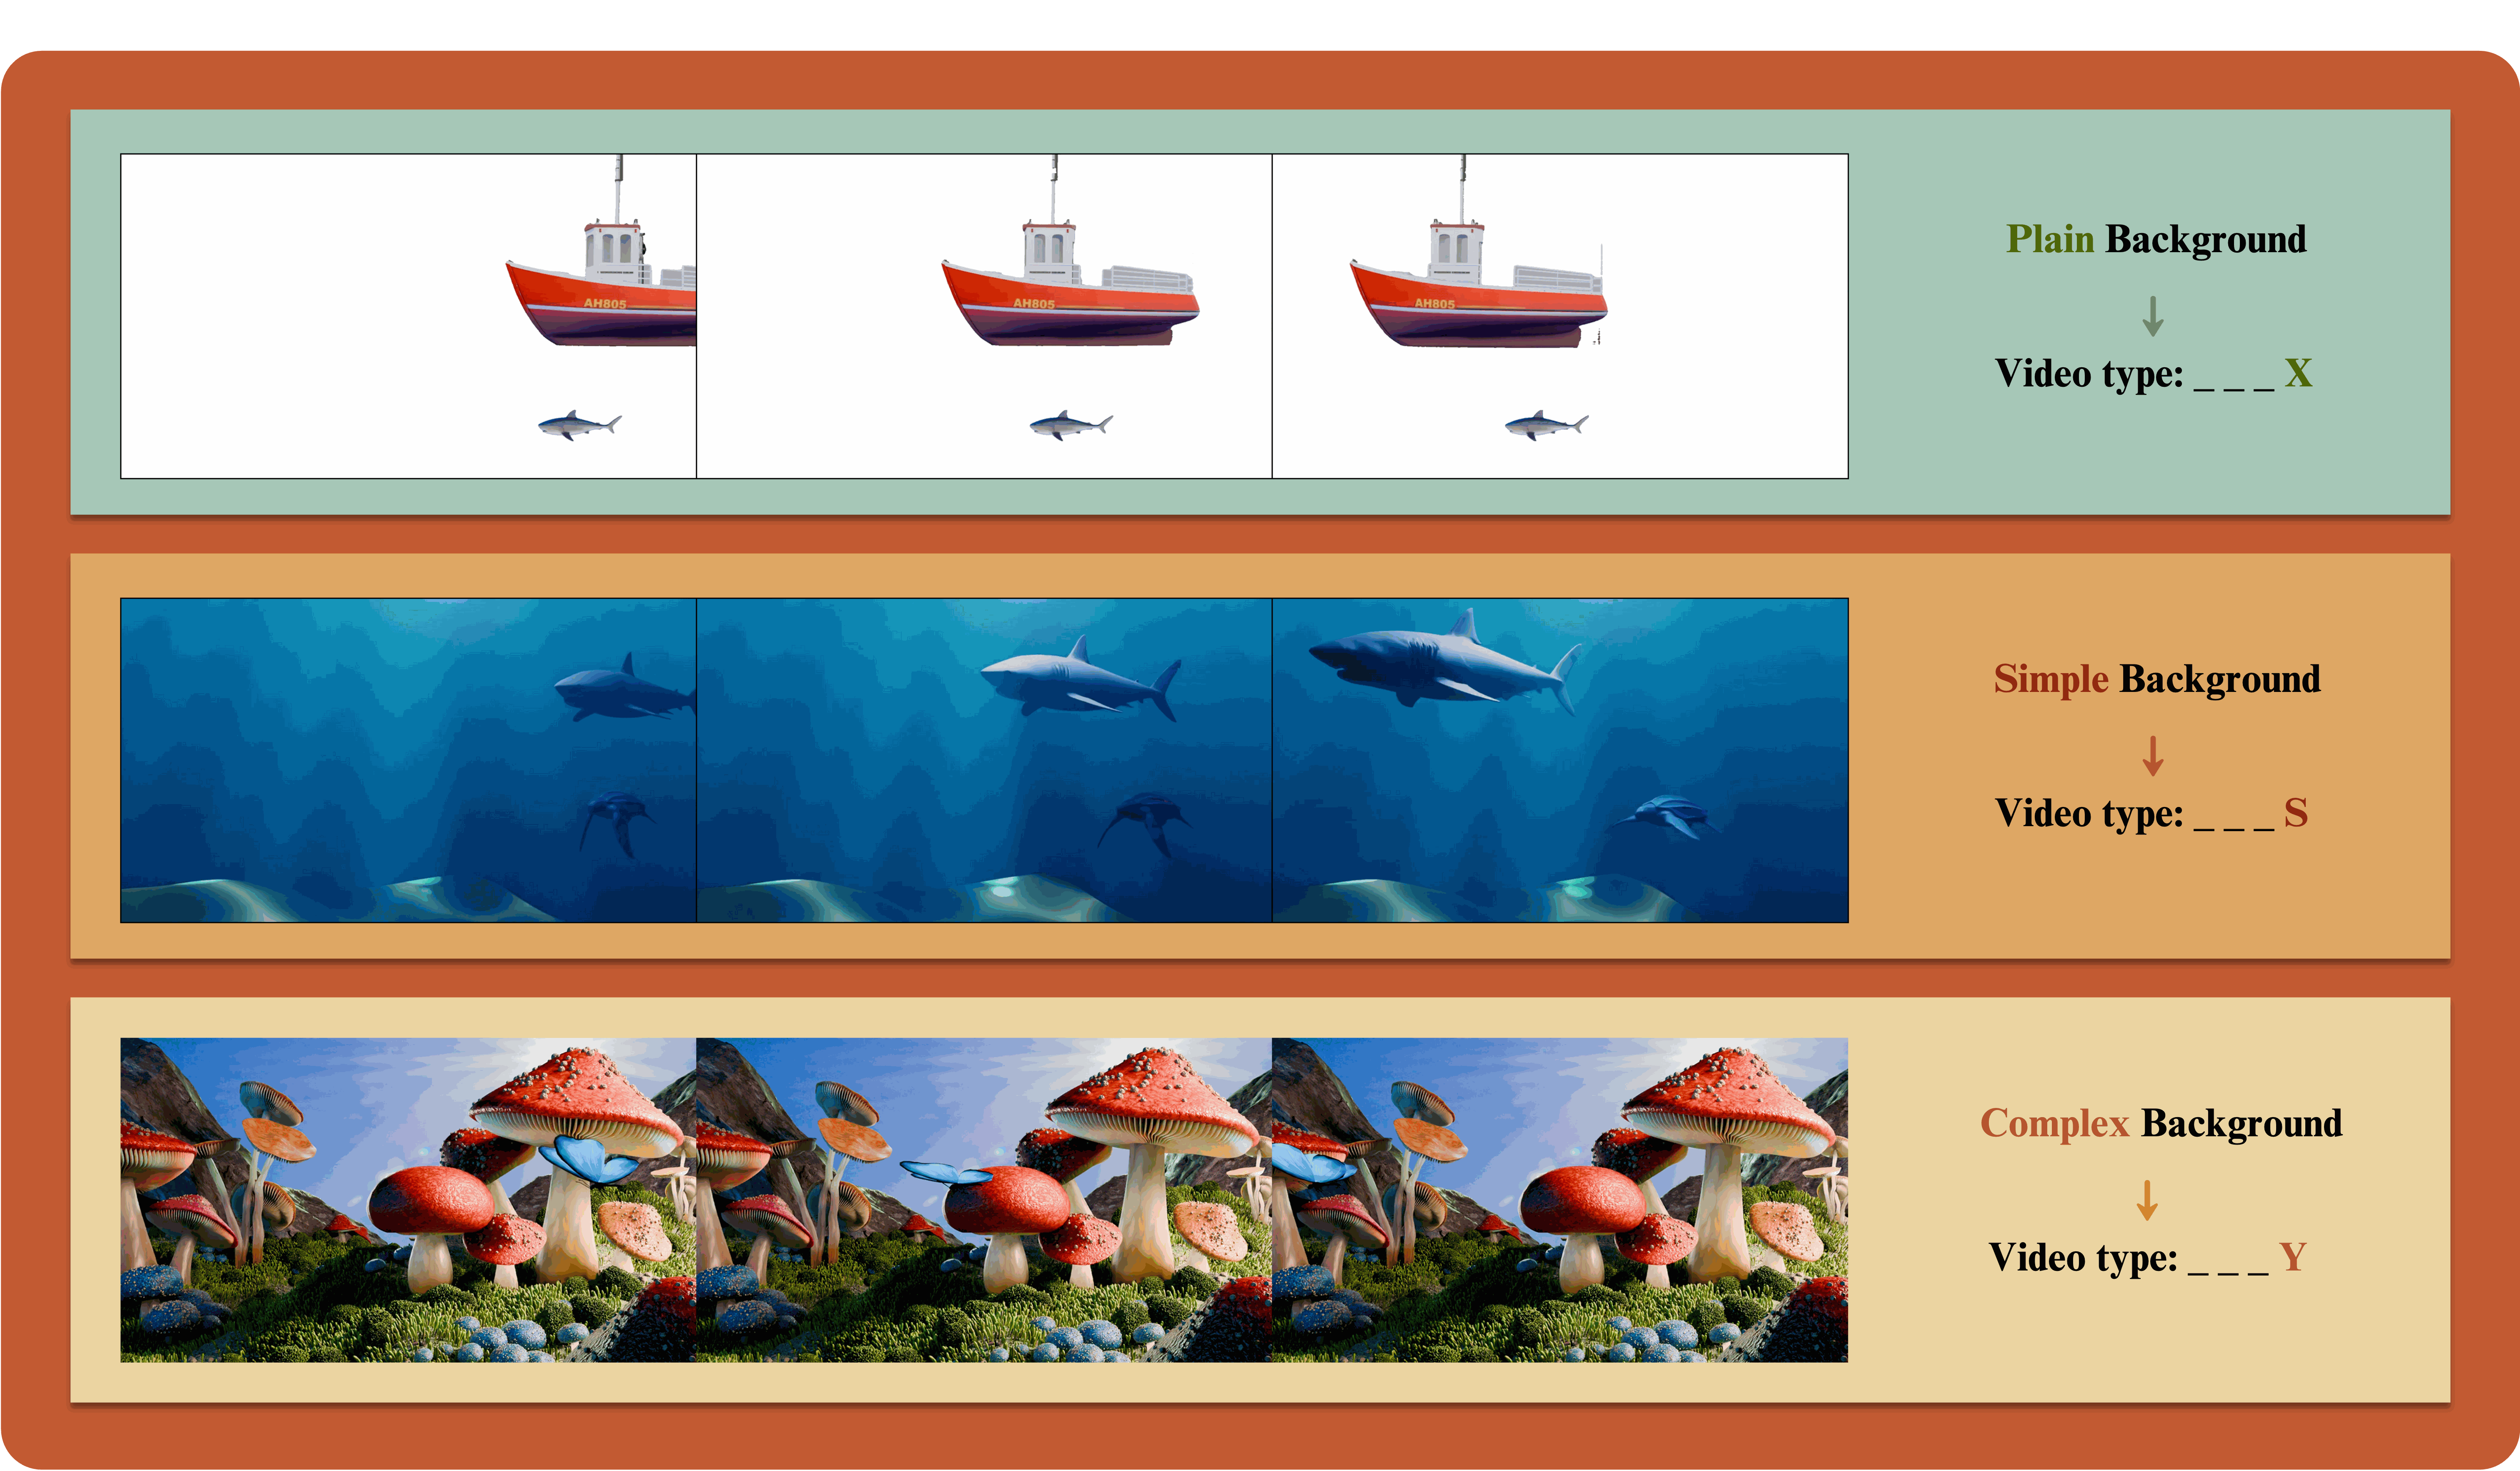
\includegraphics[width=0.99\linewidth]{sec/images/XSC2.png}
    \caption{\textbf{Examples of X/S/C scene.}}
    \label{fig:X/S/C_scene}
\end{figure*}

Putting these components together, for example, a code such as \texttt{A3MC} indicates that the video (i) targets the acceleration prior (\texttt{A}), (ii) is rendered as a 3D video (\texttt{3}), (iii) is labeled as a multiple-object setting (\texttt{M}) because at least one inference question asks about an object different from the one whose acceleration prior is defined, and (iv) uses a complex background.

\subsubsection{Quantitative breakdown of video types.}
To complement the qualitative description above, we now provide a quantitative summary of how clips are distributed across the four-character codes. The benchmark contains 569 videos in total, of which 328 are \texttt{2D} and 241 are \texttt{3D}, yielding an approximately 4:3 split between planar and volumetric setups (about 58\% \texttt{2D} and 42\% \texttt{3D}). This ensures that both \texttt{2D} and \texttt{3D} configurations are substantially represented rather than the dataset being dominated by a single family of scenes. \autoref{tab:2d3d-summary} reports the corresponding counts for each individual code and for the \texttt{2D} versus \texttt{3D} groups.
By construction, combining three physical priors (\texttt{S} / \texttt{V} / \texttt{A}), two dimensionalities (\texttt{2} / \texttt{3}), two object settings (\texttt{S} / \texttt{M}), and three background types (\texttt{X} / \texttt{S} / \texttt{C}) yields 36 distinct four-character codes, and all 36 appear in the dataset. For \texttt{2D} videos, the codes are
\texttt{A2SX, A2SS, A2SC, A2MX, A2MS, A2MC,
S2SX, S2SS, S2SC, S2MX, S2MS, S2MC,
V2SX, V2SS, V2SC, V2MX, V2MS, V2MC};
for \texttt{3D} videos, the codes are
\texttt{A3SX, A3SS, A3SC, A3MX, A3MS, A3MC,
S3SX, S3SS, S3SC, S3MX, S3MS, S3MC,
V3SX, V3SS, V3SC, V3MX, V3MS, V3MC}.
Each code is instantiated by at least 4 clips, so even the smallest categories have non-trivial support. The largest corpus (\texttt{V2MC} in our current dataset) contains 51 clips. Across all 36 codes, per-code counts range from 4 to 51 clips, with the majority lying between 5 and 35. This distribution avoids both extremely rare ``one-off'' configurations and a few overwhelmingly frequent ones. The precise per-code counts are given in \autoref{tab:2d3d-summary}.
\autoref{tab:2d3d-summary} also details how each video is obtained. The \texttt{Blender} column counts fully synthetic clips rendered directly in \texttt{Blender} from our own scenes, contributing 300 videos. The \texttt{Internet} column counts 72 clips sourced from existing online footage that we curate and annotate. The \texttt{Captured} column counts 112 clips that we record ourselves (for example, using handheld cameras or screen recordings). The \texttt{Segmented} column counts 85 clips created by segmenting foreground objects from source footage and compositing them into new backgrounds. For each four-character code, the Total column gives the number of clips that realize that configuration. Taken together, these statistics in \autoref{tab:2d3d-summary} show that the dataset spans all intended configurations, with each category populated by multiple clips and supported by a mix of blender-rendered, internet-sourced, captured, and segmented videos.

\begin{table*}[t]
\centering
\small
\renewcommand{\arraystretch}{1.1}
\begin{tabular}{l | l r r r r r r}
\toprule
2D/3D & \texttt{Video Type} & \texttt{Blender} & \texttt{Internet} & \texttt{Captured} & \texttt{Segmented} & \texttt{Total} & 2D/3D Total \\
\midrule

2D & \texttt{A2SX} & 0 & 0 & 0 & 11 & 11 &  \\
   & \texttt{A2SS} & 10 & 6 & 0 & 0  & 16 &  \\
   & \texttt{A2SC} & 10 & 5 & 0 & 0  & 15 &  \\
   & \texttt{A2MX} & 6 & 0 & 1 & 8  & 15 &  \\
   & \texttt{A2MS} & 14 & 0 & 1 & 0 & 15 &  \\
   & \texttt{A2MC} & 17 & 2 & 1 & 0 & 20 &  \\
   & \texttt{S2SX} & 0 & 0 & 0 & 10 & 10 & \\
   & \texttt{S2SS} & 10 & 5 & 0 & 0 & 15 & \\
   & \texttt{S2SC} & 7 & 8 & 0 & 0 & 15 & \\
   & \texttt{S2MX} & 8 & 0 & 0 & 8 & 16 & \\
   & \texttt{S2MS} & 11 & 3 & 0 & 0 & 14 & \\
   & \texttt{S2MC} & 16 & 20 & 0 & 0 & 36 & \\
   & \texttt{V2SX} & 2 & 0 & 0 & 9 & 11 & \\
   & \texttt{V2SS} & 10 & 7 & 0 & 0 & 17 & \\
   & \texttt{V2SC} & 10 & 8 & 0 & 0 & 18 & \\
   & \texttt{V2MX} & 13 & 0 & 0 & 7 & 20 & \\
   & \texttt{V2MS} & 13 & 0 & 0 & 0 & 13 & \\
   & \texttt{V2MC} & 43 & 8 & 0 & 0 & 51 & \\
\hline
   &       &   &   &   &   &    & 328 \\
\midrule

3D & \texttt{A3SX} & 2 & 0 & 6 & 1  & 9  &  \\
   & \texttt{A3SS} & 2 & 0 & 9 & 0  & 11 &  \\
   & \texttt{A3SC} & 3 & 0 & 7 & 0  & 10 &  \\
   & \texttt{A3MX} & 1 & 0 & 4 & 2  & 7  &  \\
   & \texttt{A3MS} & 3 & 0 & 4 & 0  & 7  &  \\
   & \texttt{A3MC} & 22 & 0 & 4 & 0 & 26 &  \\
   & \texttt{S3SX} & 1 & 0 & 8 & 2  & 11 & \\
   & \texttt{S3SS} & 2 & 0 & 8 & 0  & 10 & \\
   & \texttt{S3SC} & 2 & 0 & 8 & 0  & 10 & \\
   & \texttt{S3MX} & 0 & 0 & 9 & 13 & 22 & \\
   & \texttt{S3MS} & 1 & 0 & 10 & 0 & 11 & \\
   & \texttt{S3MC} & 24 & 0 & 10 & 0 & 34 & \\
   & \texttt{V3SX} & 3 & 0 & 2 & 0  & 5  &  \\
   & \texttt{V3SS} & 2 & 0 & 2 & 0  & 4  &  \\
   & \texttt{V3SC} & 3 & 0 & 2 & 0  & 5  &  \\
   & \texttt{V3MX} & 2 & 0 & 5 & 14 & 21 & \\
   & \texttt{V3MS} & 3 & 0 & 5 & 0  & 8  &  \\
   & \texttt{V3MC} & 24 & 0 & 6 & 0 & 30 & \\
\hline
   &       &   &   &   &   &    & 241 \\
\midrule
Total &      & 300 & 72 & 112 & 85 & 569 & 569 \\
\bottomrule
\end{tabular}
\caption{\textbf{Statistics of videos}.}
\label{tab:2d3d-summary}
\end{table*}


\section{Details of Data Collection}

\subsection{Blender Simulation}

\subsubsection{Blender Toolkits and Asset Sources}
\label{subsec:blender_toolkits}

\noindent\textbf{Asset sources and selection.}
We construct Blender scenes using 3D assets sourced from online repositories,
primarily BlenderKit and Sketchfab. We deliberately use these two libraries for
complementary purposes: BlenderKit mainly provides complex themed environments
that serve as background layouts, whereas Sketchfab mainly provides rigged and
animated foreground objects whose motions can be reused with minimal manual
keyframing.

\noindent\textbf{BlenderKit for complex themed environments.}
BlenderKit is a community-driven asset library that is tightly integrated into
Blender’s interface and offers a large collection of render-ready models,
materials, High Dynamic Range Images(HDRIs), brushes, and complete scenes that can be searched and
inserted directly from within Blender. In our pipeline, we primarily rely on
BlenderKit for complex “themed” environments, such as indoor rooms, streets, architectural spaces, and other richly cluttered layouts at both small and large spatial scales. These pre-built scenes typically include coherent lighting, materials, and background geometry (for example, furniture, buildings, and vegetation), which allows us to quickly instantiate diverse indoor and outdoor environments without having to model every object or compose every layout from scratch. This substantially reduces the authoring effort for environment design while still giving us control over camera placement, object insertion, and motion trajectories.

\noindent\textbf{Sketchfab for rigged and animated foreground objects.} Sketchfab is a large community platform for hosting and distributing 3D content, including many rigged and animated models across categories such as animals, vehicles, and articulated characters. In our work, we mainly use Sketchfab to obtain foreground objects that already come with a skeleton rig and a small set of reusable animation clips. Typical examples include wing-flapping cycles for flying birds (such as eagles spreading and flapping their wings) and swimming cycles for fish with realistic body undulation. Instead of manually keyframing these motions, we can directly reuse or lightly retarget the provided animations in our scenes. This makes it much easier to populate environments with moving agents whose motion is visually plausible, while significantly reducing the time spent on low-level animation authoring.

\noindent\textbf{Licensing and reuse.} For both BlenderKit and Sketchfab, we restrict ourselves to assets whose licenses explicitly allow reuse and modification in works. These licensing choices ensure that all assets in our dataset are used in a copyright-compliant way and that future researchers can reconstruct our pipeline using the same publicly available resources.

\begin{figure*}[h]
    \centering
    \includegraphics[width=\linewidth]{sec/images/collision.jpg}
    \caption{\textbf{Physics-driven example.} 
    A bowling ball collides with pins under Newtonian simulation. 
    The motion and resulting trajectories arise directly from rigid-body dynamics and elastic collisions, making this clip representative of our force-based motion category.}
    \label{fig:physics_example}
\end{figure*}

\begin{figure*}[h]
    \centering
    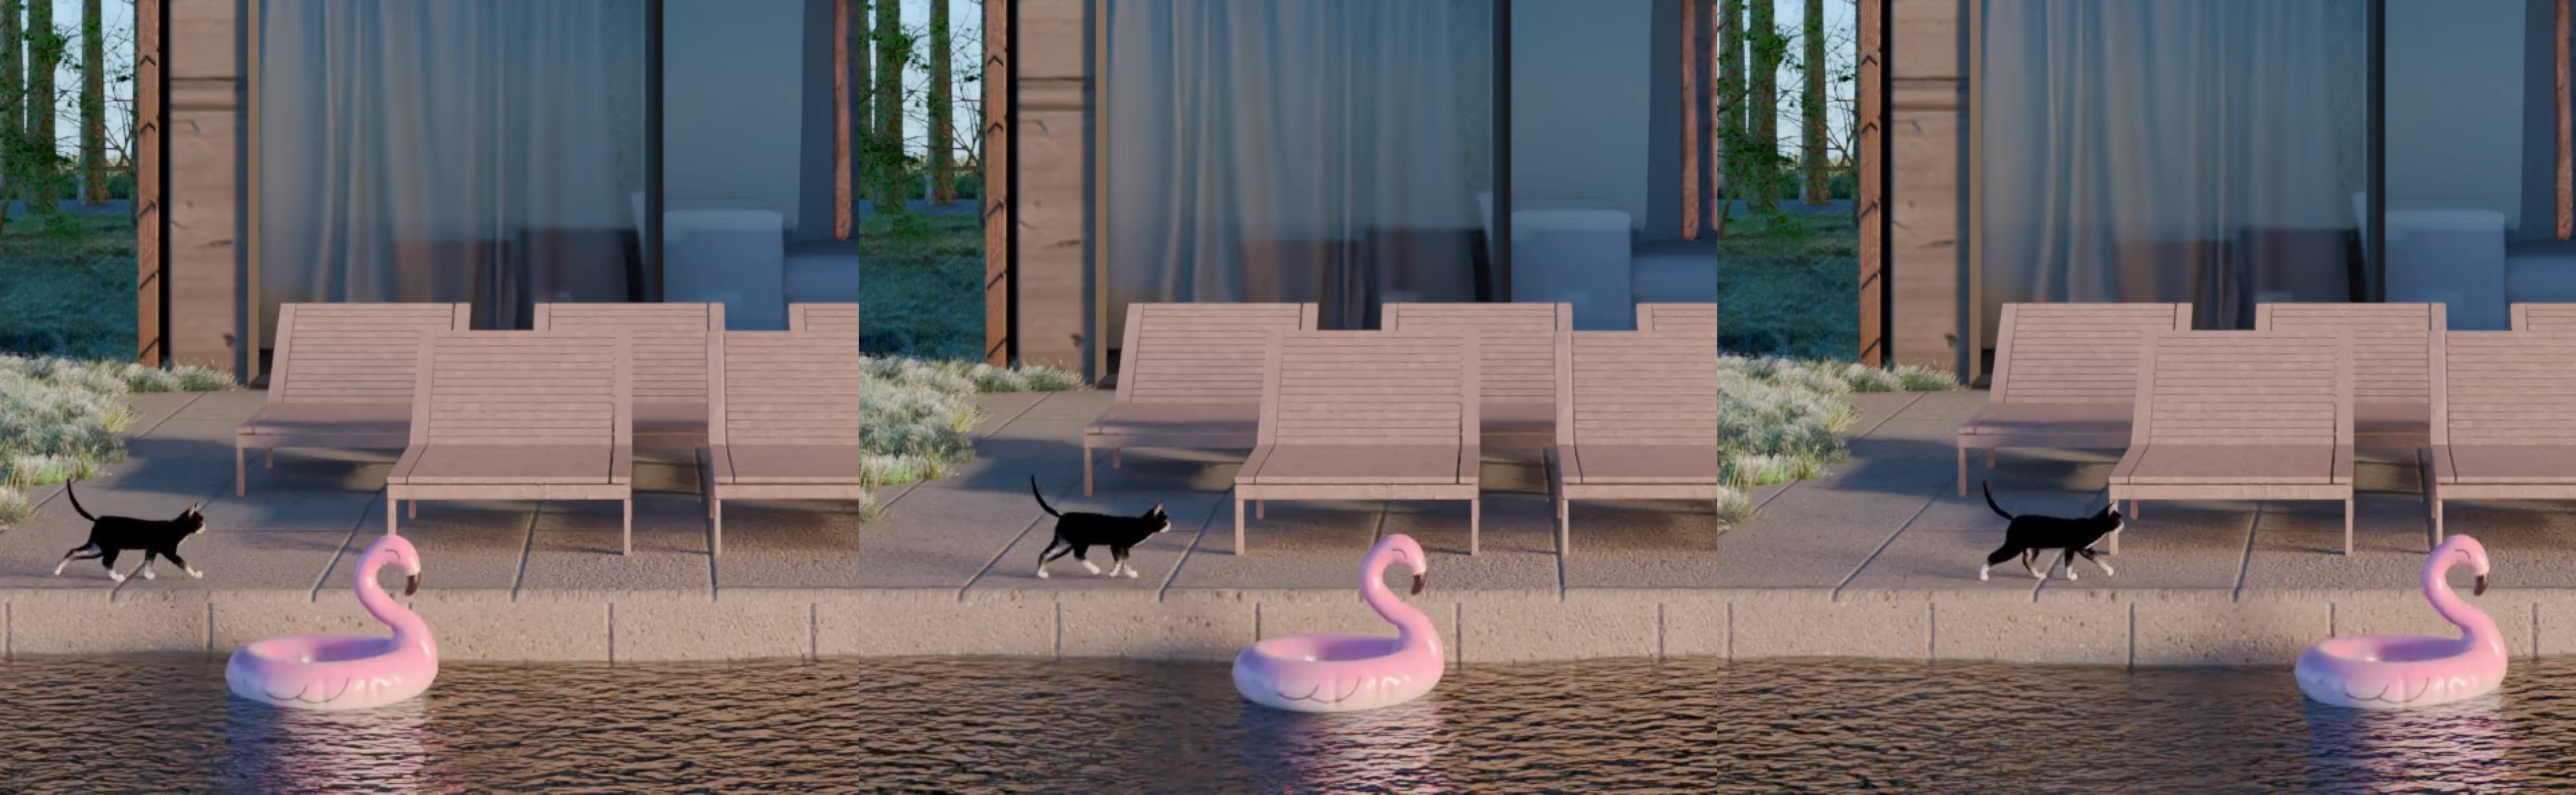
\includegraphics[width=\linewidth]{sec/images/swimring.jpg}
    \caption{\textbf{Keyframed example.} 
    The floating swim ring follows a manually authored animation curve rather than buoyancy, drag, or wind forces. 
    Its trajectory is visually plausible but not physically derived, representing our keyframed motion category.}
    \label{fig:keyframe_example}
\end{figure*}

\begin{figure*}[h]
    \centering
    \includegraphics[width=\linewidth]{sec/images/curve.png}
    \caption{\textbf{Keyframed animation-curve example.} 
    The animation curve controlling the swim ring in \autoref{fig:keyframe_example}. 
    The ring moves forward along a manually authored trajectory, while small randomized perturbations in translation and rotation are added to imitate the visual appearance of floating motion.}
    \label{fig:animation_curve_example}
\end{figure*}

\begin{figure}[h]
    \centering
    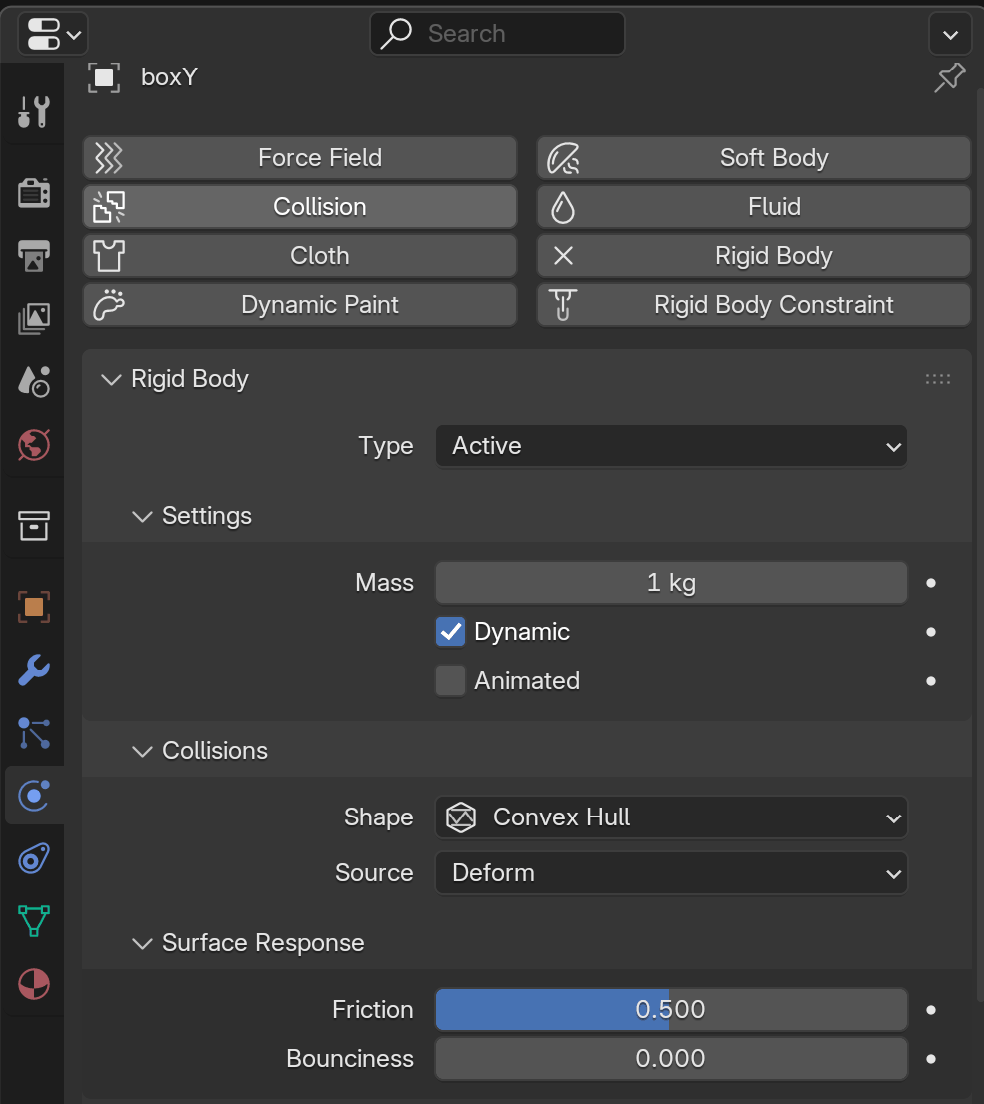
\includegraphics[width=\linewidth]{sec/images/rigidbody.png}
    \caption{\textbf{Physics-driven rigid-body example.}
    Rigid-body simulation of objects such as the bowling pins reacting to the impact of an incoming ball in \autoref{fig:physics_example}.
    The pins' motion, tipping, and scattering are governed entirely by Newtonian dynamics and collision responses within the physics engine.}
    \label{fig:rigid_body_example}
\end{figure}


\subsubsection{Two Motion Simulation Types}
\label{subsec: MotionType}
The Blender-generated portion of our dataset contains two complementary categories of motion, reflecting the major paradigms of movement in computer graphics and physics-based animation.

\noindent\textbf{(1) Keyframed Motion.} 
Examples of this category are shown in \autoref{fig:keyframe_example}.
This category includes humans, animals, and other objects whose motion is defined using rigged skeletons or keyframed animation curves shown in \autoref{fig:animation_curve_example}. Because these trajectories are authored manually rather than produced through physical simulation, they are {visually plausible but not physically constrained}.

A key implication is that the resulting motion does not necessarily obey real-world physical laws. For example, in the lunar-walking scene (\autoref{fig:astronaut_scene}), the astronaut’s push-off, airtime, and landing motion are shaped by artist-edited animation curves. Although the motion is loosely inspired by reduced lunar gravity, we do not compute the animation using the Moon's gravitational constant nor derive the trajectory from force-based simulation. These sequences should therefore be interpreted as {perceptually reasonable approximations} of motion rather than physically calibrated ground truth.

\noindent\textbf{(2) Physics-Driven / Force-Based Motion.}
Examples of this category are shown in \autoref{fig:physics_example}.
This category consists of rigid bodies (shown in \autoref{fig:rigid_body_example}) moving directly under Newtonian dynamics. Their trajectories are generated by applying explicit forces (e.g., gravity, impulses) inside a physics engine or by specifying analytical kinematic profiles (e.g., constant velocity, uniform acceleration, projectile motion). These clips yield clean and physically interpretable motion, allowing us to provide exact ground-truth displacement, velocity, and acceleration.

For all videos in this category, we explicitly state the forces or kinematic parameters involved, and these values constitute part of the known prior information for each question.

\noindent\textbf{Clarifying Prior Knowledge vs.\ Visual Assumptions.}
In an era where videos may originate from real capture, simulation software, procedural animation, or generative models, visual motion alone does not guarantee adherence to physical laws. Accordingly, VLMs should reason strictly based on the prior conditions we provide, rather than relying on pretrained assumptions about how objects “should” move.

When prior information explicitly specifies a force or acceleration (e.g., “the object accelerates at $2.5\,\mathrm{m/s^2}$”), that value serves as authoritative ground truth. When such information is not given, the model should not infer physical constants, such as Earth's gravity, only from the visual appearance of the motion. Because our dataset includes diverse simulated and animated sequences, correct reasoning requires using only the provided priors, not assumed real-world physics.

\subsubsection{Blender Videos Construction}
\label{subsec:blendervideo_construction}

\noindent\textbf{Quantitative Overview.} In the Blender subset, we start from approximately 125 distinct base 3D models and 81 base scenes. From these bases, we generate 312 unique Blender video clips. Beyond simply increasing the size of the dataset, Blender enables us to construct diverse scenes and controlled trajectories of objects in simplified environments. Because these scenes are generated procedurally, we can precisely specify object sizes, positions, and kinematics via scripts and directly compute accurate ground-truth physical quantities for each clip. As a result, the Blender subset is not only large, but also covers a broad spectrum of scene scales and motions under tight experimental control.

\noindent\textbf{Scene Construction.} We construct a diverse collection of synthetic scenes to broaden the range of physical situations represented in the benchmark. Specifically, we design both everyday indoor spaces (e.g., rooms with furniture and household objects, see \autoref{fig:indoor_scene}) and outdoor spaces (e.g., natural environments with varied terrain, vegetation, and water, see \autoref{fig:outdoor_scene}). These scenes differ in layout, depth structure, and illumination, so that models must handle physical reasoning under heterogeneous visual conditions rather than overfitting to a single canonical setting.

\begin{figure*}[ht!]
    \centering
    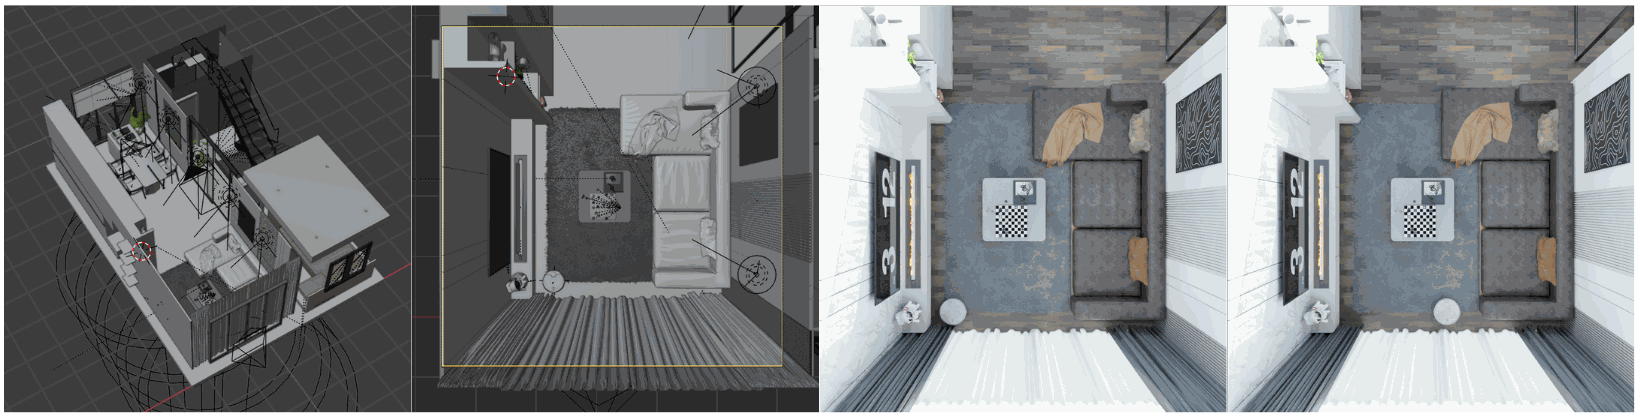
\includegraphics[width=0.99\linewidth]{sec/images/indoor_scene.png}
    \caption{\textbf{Examples of indoor scene.}}
    \label{fig:indoor_scene}
\end{figure*}

\begin{figure*}[ht!]
    \centering
    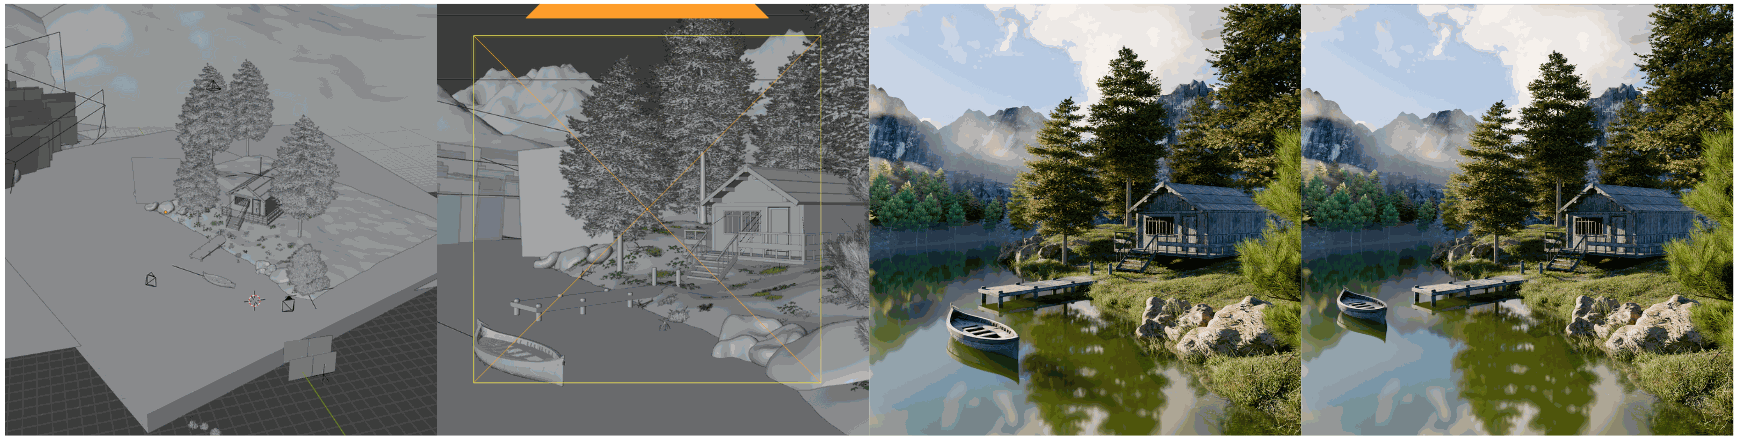
\includegraphics[width=0.99\linewidth]{sec/images/outdoor_scene.png}
    \caption{\textbf{Examples of outdoor scene.}}
    \label{fig:outdoor_scene}
\end{figure*}

Beyond such everyday environments, we also include scenes that are difficult or impossible to capture, measure, or systematically manipulate in the real world. Examples include microscopic settings (e.g., red blood cells moving through a vessel, see \autoref{fig:microscopic_scene}), extraterrestrial scenarios (e.g., astronaut motion on the Moon, see \autoref{fig:astronaut_scene}), and more. 

\begin{figure*}[ht!]
    \centering
    \includegraphics[width=0.99\linewidth]{sec/images/complex_red_blood_cell.png}
    \caption{\textbf{Examples of microscopic scene.}}
    \label{fig:microscopic_scene}
\end{figure*}

\begin{figure*}[ht!]
    \centering
    \includegraphics[width=0.99\linewidth]{sec/images/astronaut.png}
    \caption{\textbf{Examples of extraterrestrial scene.}}
    \label{fig:astronaut_scene}
\end{figure*}

Starting from base assets and scenes, we explicitly control geometry, lighting, and background complexity to generate families of videos that fall into different categories in our taxonomy. For instance, in the red-blood-cell scene (\autoref{fig:building_x_scene}), we derive a 3MX-style variant by removing the vessel wall, discarding all but two target cells, and replacing the background with a uniform RGB field. Using the same procedure, as shown in the \autoref{fig:building_s_scene} we construct simple-background versions of more complex scenes by simplifying clutter while keeping coarse structural cues (e.g., horizon lines, major surfaces, object structures) and realistic lighting. 

It is important to note that, although we present several examples that appear to reuse the same underlying scene. In practice, not all plain-background videos and simple-background videos are reused across conditions. In addition, we also include videos that are uniquely constructed to appear only in the plain-background condition or only in the simple-background condition. This design choice is intended to increase the diversity of the video data. Reusing identical base scenes improves the efficiency of dataset construction, but it may also introduce potential biases or unwanted correlations when evaluating VLMs, so we deliberately balance such reuse with the creation of novel, non-paired scenes.

\begin{figure*}[ht!]
    \centering
    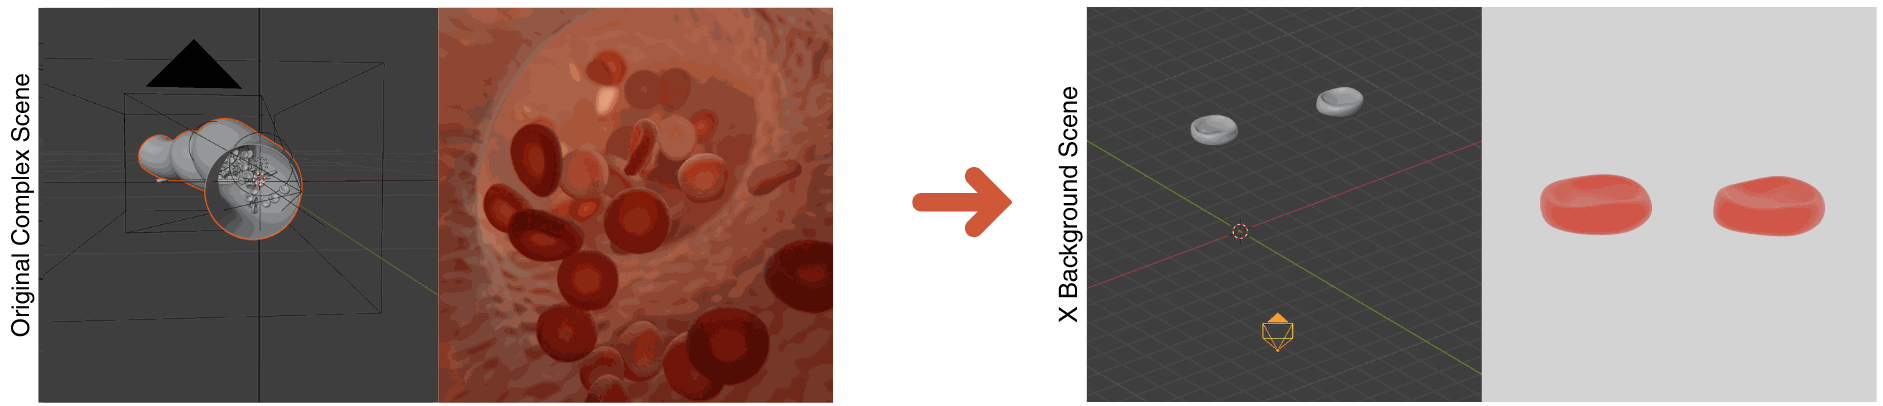
\includegraphics[width=0.99\linewidth]{sec/images/simplify_to_x_bg.png}
    \vspace{-0.5em}
    \caption{\textbf{Examples of building X background scene.}}
    \label{fig:building_x_scene}
\end{figure*}

\begin{figure*}[ht!]
    \centering
    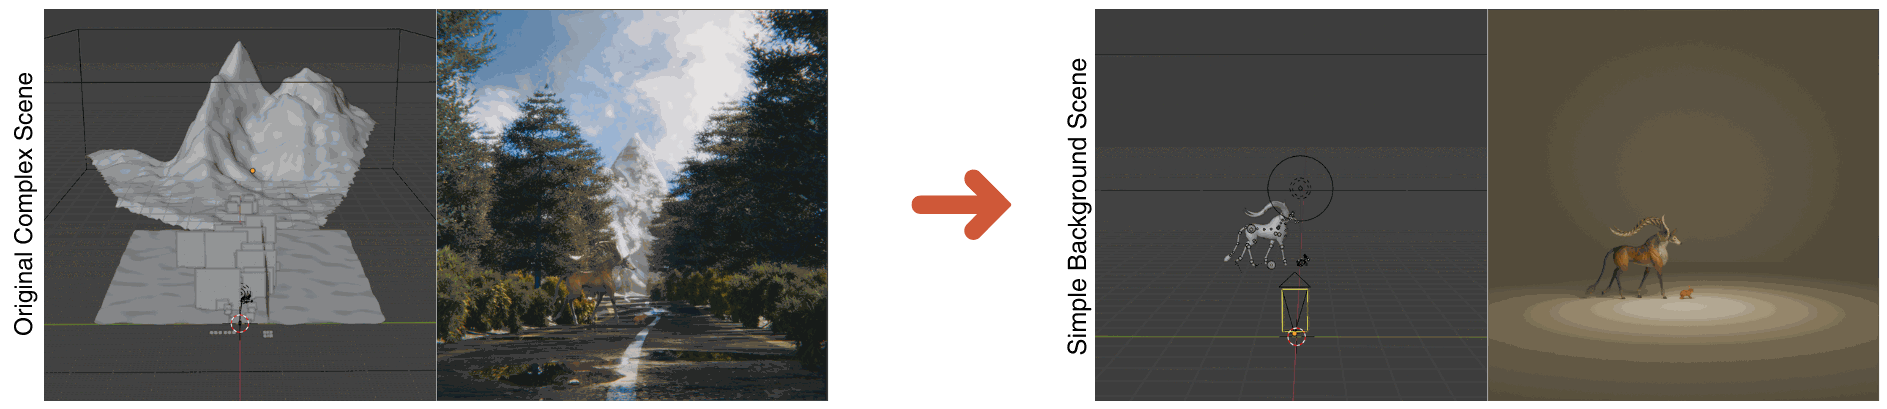
\includegraphics[width=0.99\linewidth]{sec/images/simplify_to_s_bg.png}
    \vspace{-0.5em}
    \caption{\textbf{Examples of building S background scene.}}
    \label{fig:building_s_scene}
\end{figure*}


For the objects in each scene, we specify target object sizes, velocities, and accelerations using real-world statistics gathered from online references (e.g., typical dimensions and speeds of vehicles, animals, and more). Whenever possible, moving objects are modeled at real-world scale; in rare cases where real-world-scale objects yield motion trajectories that are barely discernible in the rendered videos, we apply uniform scaling to increase perceptual visibility while preserving the underlying physical relationships.

An example is the “ice cube falling into a cup” scene illustrated in the \autoref{fig:scaled_scene}. If we model the cup and cube at their real-world dimensions, the cube traverses the camera frustum in essentially a single frame, making its falling trajectory almost invisible to observers and thus providing little signal for quantitative evaluation. To address this, we uniformly enlarge both the cup and the ice cube by a factor of 10. After scaling, the cube remains visible from frame 11 to 22, and the rendered video reveals a clear multi-frame trajectory. This controlled rescaling not only makes the motion measurable but also allows us to probe whether VLMs recover physical quantities from the observed kinematics given the priors specified in the prompt, or whether they instead rely predominantly on generic pre-trained knowledge and commonsense expectations about how such objects “should” behave.

\begin{figure*}[ht!]
    \centering
    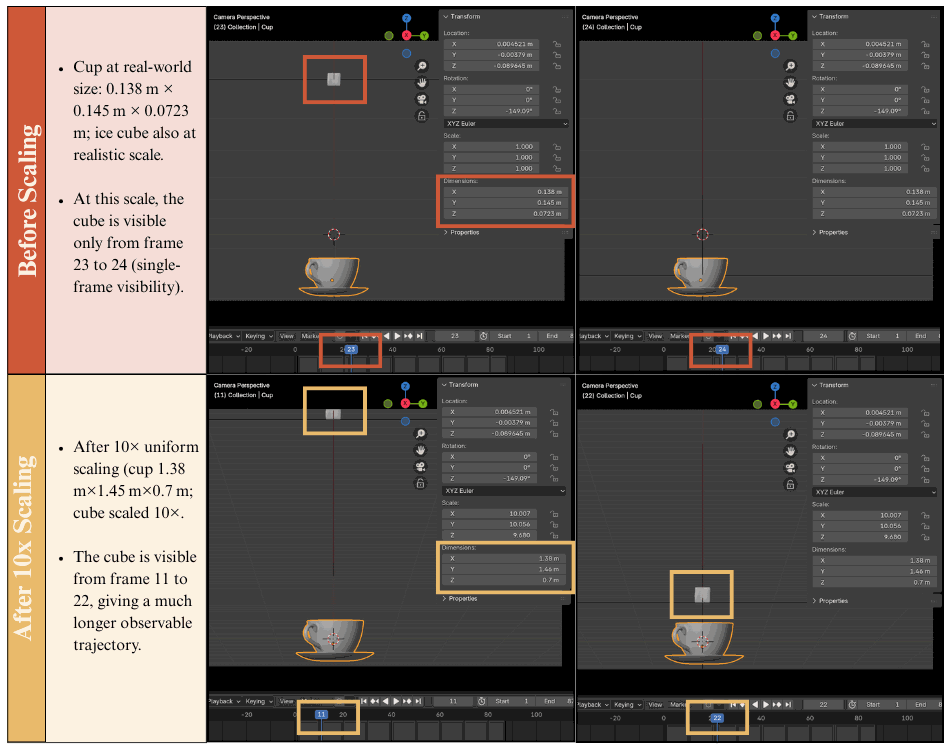
\includegraphics[width=0.99\linewidth]{sec/images/scaled_scene.png}
    \caption{\textbf{Examples of scaled scene.}}
    \label{fig:scaled_scene}
\end{figure*}

\noindent\textbf{Object Motion Design and Implementation.}
As discussed in \autoref{subsec: MotionType}, our motion design follows two main paradigms: keyframed motion and physics-driven motion. The construction of physics-driven scenes is illustrated in \autoref{fig:physics_example}. For the keyframed cases, in addition to manual editing in the Graph Editor, we also use scripts to automate the animation process.

We distinguish two main classes of scripted motion: (i) analytic one-dimensional motion along a single axis, and (ii) curve-following motion along human-designed paths.

For analytic 1D motion, we explicitly encode standard kinematic equations and bake the resulting trajectories as keyframes. Given an object with initial world-space position $\mathbf{x}_0$, a target duration $T$, and a desired acceleration $a$ along the $-Y$ axis, our script iterates over frames $f$ and computes the physical time
\[
t = \frac{f - \texttt{START\_FRAME}}{\texttt{FPS}}.
\]

The corresponding displacement is computed using the constant-acceleration formula
\[
s(t) = \tfrac{1}{2} a t^{2}.
\]

\begin{minted}[
  fontsize=\footnotesize,
  linenos,
  frame=lines,
  framesep=2mm,
  baselinestretch=1.0,
  breaklines,
  bgcolor=black!2
]{python}
disp_y = 0.5 * ACCEL * (t ** 2)
new_y  = start_loc.y - disp_y
obj.location = Vector((start_loc.x, new_y, start_loc.z))
obj.keyframe_insert(data_path="location", index=-1, frame=f)
\end{minted}


% \begin{quote}
% {\footnotesize
% \begin{verbatim}
% disp_y = 0.5 * ACCEL * (t ** 2)
% new_y  = start_loc.y - disp_y
% obj.location = Vector((start_loc.x, new_y, start_loc.z))
% obj.keyframe_insert(data_path="location", index=-1, frame=f)
% \end{verbatim}
% }
% \end{quote}

This directly realizes $s(t)=\tfrac{1}{2} a t^{2}$ in world coordinates. For constant-velocity motion, we instead use the linear relation:
\[
s(t) = v t,
\]
implemented via

\begin{minted}[
  fontsize=\footnotesize,
  linenos,
  frame=lines,
  framesep=2mm,
  baselinestretch=1.0,
  breaklines,
  bgcolor=black!2
]{python}
disp_y = VEL * t
new_y  = start_loc.y - disp_y
\end{minted}


while keeping the same frame loop and keyframe insertion logic. After all keyframes are written, we programmatically set each F-curve’s interpolation mode to \texttt{LINEAR}, overriding Blender’s default Bézier interpolation to ensure that the frame-to-frame displacement matches the analytically specified velocity or acceleration profile rather than being inadvertently smoothed or distorted.

For more complex motions along curved paths, we first author an approximate trajectory in Blender (e.g., by manually keyframing a car following a road or a particle moving along a spiral), and then reparameterize this path in Python to obtain physically interpretable kinematics. Concretely, we sample the object’s world-space position at each frame of the original animation:

\begin{minted}[
  fontsize=\footnotesize,
  linenos,
  frame=lines,
  framesep=2mm,
  baselinestretch=1.0,
  breaklines,
  bgcolor=black!2
]{python}
positions = []
for f in range(frame_start, frame_end + 1):
    scene.frame_set(f)
    pos = obj.matrix_world.translation.copy()
    positions.append(pos)
\end{minted}

% \begin{quote}
% {\footnotesize
% \begin{verbatim}
% positions = []
% for f in range(frame_start, frame_end + 1):
%     scene.frame_set(f)
%     positions.append(obj.matrix_world.translation.copy())
% \end{verbatim}
% }
% \end{quote}

We then compute the cumulative arc length along this polyline.

\begin{minted}[
  fontsize=\footnotesize,
  linenos,
  frame=lines,
  framesep=2mm,
  baselinestretch=1.0,
  breaklines,
  bgcolor=black!2
]{python}
distances = [0.0]
for i in range(1, len(positions)):
    d = (positions[i] - positions[i-1]).length
    distances.append(distances[-1] + d)
total_length = distances[-1]
duration     = (frame_end - frame_start) / fps
\end{minted}
\noindent We then derive a desired kinematic profile in terms of traveled distance $s(t)$ along the curve. For constant-speed motion, we set $v = L/T$ with $L = \texttt{total\_length}$ and use
\[
s(t) = v t,
\]
implemented as

\begin{minted}[
  fontsize=\footnotesize,
  linenos,
  frame=lines,
  framesep=2mm,
  baselinestretch=1.0,
  breaklines,
  bgcolor=black!2
]{python}
target_dist = speed * t
\end{minted}
\noindent which corresponds to s(t)=vt. For constant-acceleration motion along the same curve, we instead use the quadratic form
\[
s(t) = v_0 t + \tfrac{1}{2} a t^{2},
\]
with user-specified $v_0$ and $a$. In both cases, for each frame we find the segment $[i-1,i]$ such that
\[
\texttt{distances}[i-1] \le s(t) \le \texttt{distances}[i],
\]
and linearly interpolate between the sampled positions:

\begin{minted}[
  fontsize=\footnotesize,
  linenos,
  frame=lines,
  framesep=2mm,
  baselinestretch=1.0,
  breaklines,
  bgcolor=black!2
]{python}
ratio  = (target_dist - distances[i-1]) / (distances[i] - distances[i-1])
new_loc = positions[i-1].lerp(positions[i], ratio)
obj.location = new_loc
obj.keyframe_insert(data_path="location", frame=f)
\end{minted}

Finally, as in the analytic case, all resulting keyframes are set to linear interpolation. This arc-length reparameterization scheme lets us reuse authored trajectories while imposing well-defined kinematic profiles (constant velocity, constant acceleration, or other time–distance schedules) in physical units. Together with the untouched native animations, these scripted motions give our benchmark a wide spectrum of motion patterns, from simple 1D acceleration to complex, irregular dynamics, under tight quantitative control.

\noindent\textbf{Rendering.} All Blender-generated videos in \textsc{QuantiPhy} are rendered with the Cycles and EEVEE path-tracing engine using a physically based workflow. Videos use multiple spatial resolutions, including $1920{\times}1080$ (16:9), $1080{\times}1080$ (1:1), $480{\times}960$ (vertical), as well as several additional intermediate sizes, so that models see both landscape, square, and portrait-style content. The temporal sampling is likewise heterogeneous: frame rates in the benchmark include $24$, $25$, $30$, $33$, $60$, and $120$fps. Frames are exported via FFmpeg as MP4 files with H.264 compression and a constant frame rate, without any interpolation or stabilization, so each frame aligns exactly with the simulated timeline and ground-truth annotations.

Camera parameters are also varied to increase visual diversity. Intrinsics cover a range of focal lengths from wide to normal and telephoto views, and extrinsics place the camera at different heights, offsets, and azimuth/elevation angles around the scene, producing both frontal and oblique perspectives on object motion. Lighting setups combine different environment maps and local light sources, and objects are assigned a broad set of physically based materials (e.g., diffuse, glossy, metallic, translucent), leading to diverse shading, reflection, and contrast conditions. Together, these choices give \textsc{QuantiPhy} wide coverage over resolutions, frame rates, viewpoints, and appearance statistics, while the underlying physical trajectories and numeric ground truth remain precisely controlled.



\begin{table*}[ht]
\centering
\begin{tabular}{@{}ll@{}}
\toprule
\textbf{Depth Technology}      & Time of Flight \\[3pt]
\textbf{Wavelength}            & 850\,nm \\[3pt]
\textbf{Depth Range}           & *0.25--5.46\,m (depending on depth mode) \\[3pt]
\textbf{Depth Resolution/FPS}  & Up to \(1024 \times 1024@15\) fps (WFOV), \(640 \times 576@30\) fps (NFOV) \\[3pt]
\textbf{Depth FOV}             & H \(120^\circ\) V \(120^\circ\) (WFOV), H \(75^\circ\) V \(65^\circ\) (NFOV) \\[3pt]
\textbf{RGB Resolution/FPS}    & Up to \(3840 \times 2160@25\) fps \\[3pt]
\textbf{RGB FOV}               & H \(80^\circ\) V \(51^\circ\) \\[3pt]
\textbf{Processing}            & NVIDIA Jetson Nano \\[3pt]
\textbf{IMU}                   & Supported \\
\bottomrule
\end{tabular}
\caption{\textbf{Specifications of the cameras used in our customized motion capture system.}}
\label{tab:camera}
\end{table*}


\begin{table}[ht]
\centering
\small
\setlength{\tabcolsep}{8pt}
\renewcommand{\arraystretch}{1.1}
\begin{tabular}{l l}
\toprule
Objects & Dimensions \\
\midrule
2 green tennis balls & d = 6.7 cm \\
2 pink tennis balls & d = 6.7 cm \\
2 white ping pong balls & d = 4 cm \\
1 purple yoga ball & d = 52.2 cm \\
1 soccer ball & d = 17.5 cm \\
1 basketball & d = 23.2 cm \\
1 red plastic ball & d = 7 cm \\
1 orange plastic ball & d = 5.7 cm \\
1 small whiteborad (slope) & 30.8 cm x 23.2 cm x 0.5 cm \\
1 large whiteborad & 81 cm x 60 cm x 1 cm \\
1 trashbin & 34.5 cm x 89.1 cm 59.9 cm \\
1 tape & 10.1 cm x 10.1 cm x 4.8 cm \\
1 white food box & 19.5 cm x 6.0 cm x 7.2 cm \\
stuffed toy 1 & 14.5 cm x 11 cm x 8 cm \\
stuffed toy 2 & 29.5 cm x 15.0 cm x 10.0 cm \\
stuffed toy 3 & 8.1 cm x 6.4 cm x 19.6 cm \\
1 toy cookie & 8.0 cm x 8.0 cm x 1.8 cm \\
1 cosmetic jar & 7.2 cm x 7.2 cm x 6.0 cm \\
1 glass jar & 6.8 cm x 6.8 cm x 8.5 cm \\
1 white cup & 8.6 cm x 8.6 cm x 14.5 cm \\
1 pink water bottle & 6.7 cm x 6.7 cm x 19.5 cm \\
1 marker & 13.5 cm x 0.8 cm x 0.8 cm \\
1 black pen & 14.5 cm x 1. 2 cm x 1.2 cm \\
1 green notebook & 18.6 cm x 8.8 cm x 1.5 cm \\
1 white-covered book & 12.5 cm x 19.5 cm x 2.2 cm \\
1 pencil case & 6.7 cm x 7.2 cm x 21 cm \\
1 credit card & 85.6 mm x 53.98 mm \\
1 deck of poker card & 9.8 cm x 6.3 cm x 1.8 cm \\
\bottomrule
\end{tabular}
\caption{\textbf{List of physical objects and their measured dimensions used in our lab-captured videos.}}
\label{tab:object-list}
\end{table}

\subsection{Lab Capturing}

To further complement the diversity of \textsc{QuantiPhy} with real-world data, a major part of our dataset comes from a customized motion capture system in a lab environment. Due to the nature of real-world data, lab captured videos contribute only to the category of 3D.

\noindent\textbf{MoCap setup.} 
We use four Orbbec Femto Mega cameras to construct our customized motion capture system. The specifications of the cameras are shown in \autoref{tab:camera}.

We designed two different camera setups and object arrangements in the MoCap system. The first setup covers a smaller spatial range, with the main camera placed close to the objects. In this setup, we capture motions of small objects such as a tennis ball, book, and ping pong ball moving on a desk. The second setup covers a larger range and is used to capture larger-scale motions such as basketball bouncing and accelerated motion of a trash bin. For both setups, we initialize the camera extrinsics via multi-view calibration with a checkerboard.

\noindent\textbf{Collection workflow.} 
For efficient video capture, we developed a tool with a user-friendly interface that supports synchronized recording across all four cameras. We collect videos based on a list of predefined questions. For each question, we set up the scene and objects without moving the cameras and then perform specific object motions according to the question. Three people were involved in the lab data collection workflow: one person was responsible for operating the tool (starting and pausing capture), and two people were responsible for setting up the scenes and executing the motions.

Unlike Blender simulation, capturing real-world data makes it difficult to directly manipulate specific scene parameters. We therefore manually configured the scenes to meet target conditions, such as the slope angle or the frequency of pendulum motion, using careful measurements within a set tolerance. For motions that require a controlled initial velocity, we used a motor running at s constant speed to pull the object and provide the desired initial velocity.

\noindent\textbf{Post-processing.} 
After capturing the raw videos, we obtain \texttt{.bag} files for each camera that contain the binary recordings. We follow the official camera SDK to decode the raw data. From this decoding, we obtain: (1) intrinsics for each camera, (2) timestamped RGB streams for each camera, (3) timestamped depth streams for each camera, and (4) relative extrinsics from the depth cameras to the RGB cameras. We then apply coordinate transformations to reproject the depth data into the image coordinates of the RGB videos, which allows pixel-wise depth values to be read consistently.

With aligned image coordinates, it becomes possible to read out specific depth values for target objects (with respect to the main camera). A straightforward approach is to use segmentation masks for the target object and average the depth values over the masked pixels. However, this automated approach did not work well in practice because the depth information from the camera is often incomplete and ambiguous, especially at pixels with high motion, due to hardware limitations. As a result, we could not reliably automate depth extraction for the target objects using only segmentation masks.

To ensure high-quality depth measurements, we developed a UI-based tool that overlays the transformed depth map on top of the RGB frames. The tool allows users to click on the frame to read out exact depth values from the main camera at the selected pixels. An illustration of this UI-based tool is shown in \autoref{fig:depth_annotator}.


\begin{figure*}[ht]
    \centering
    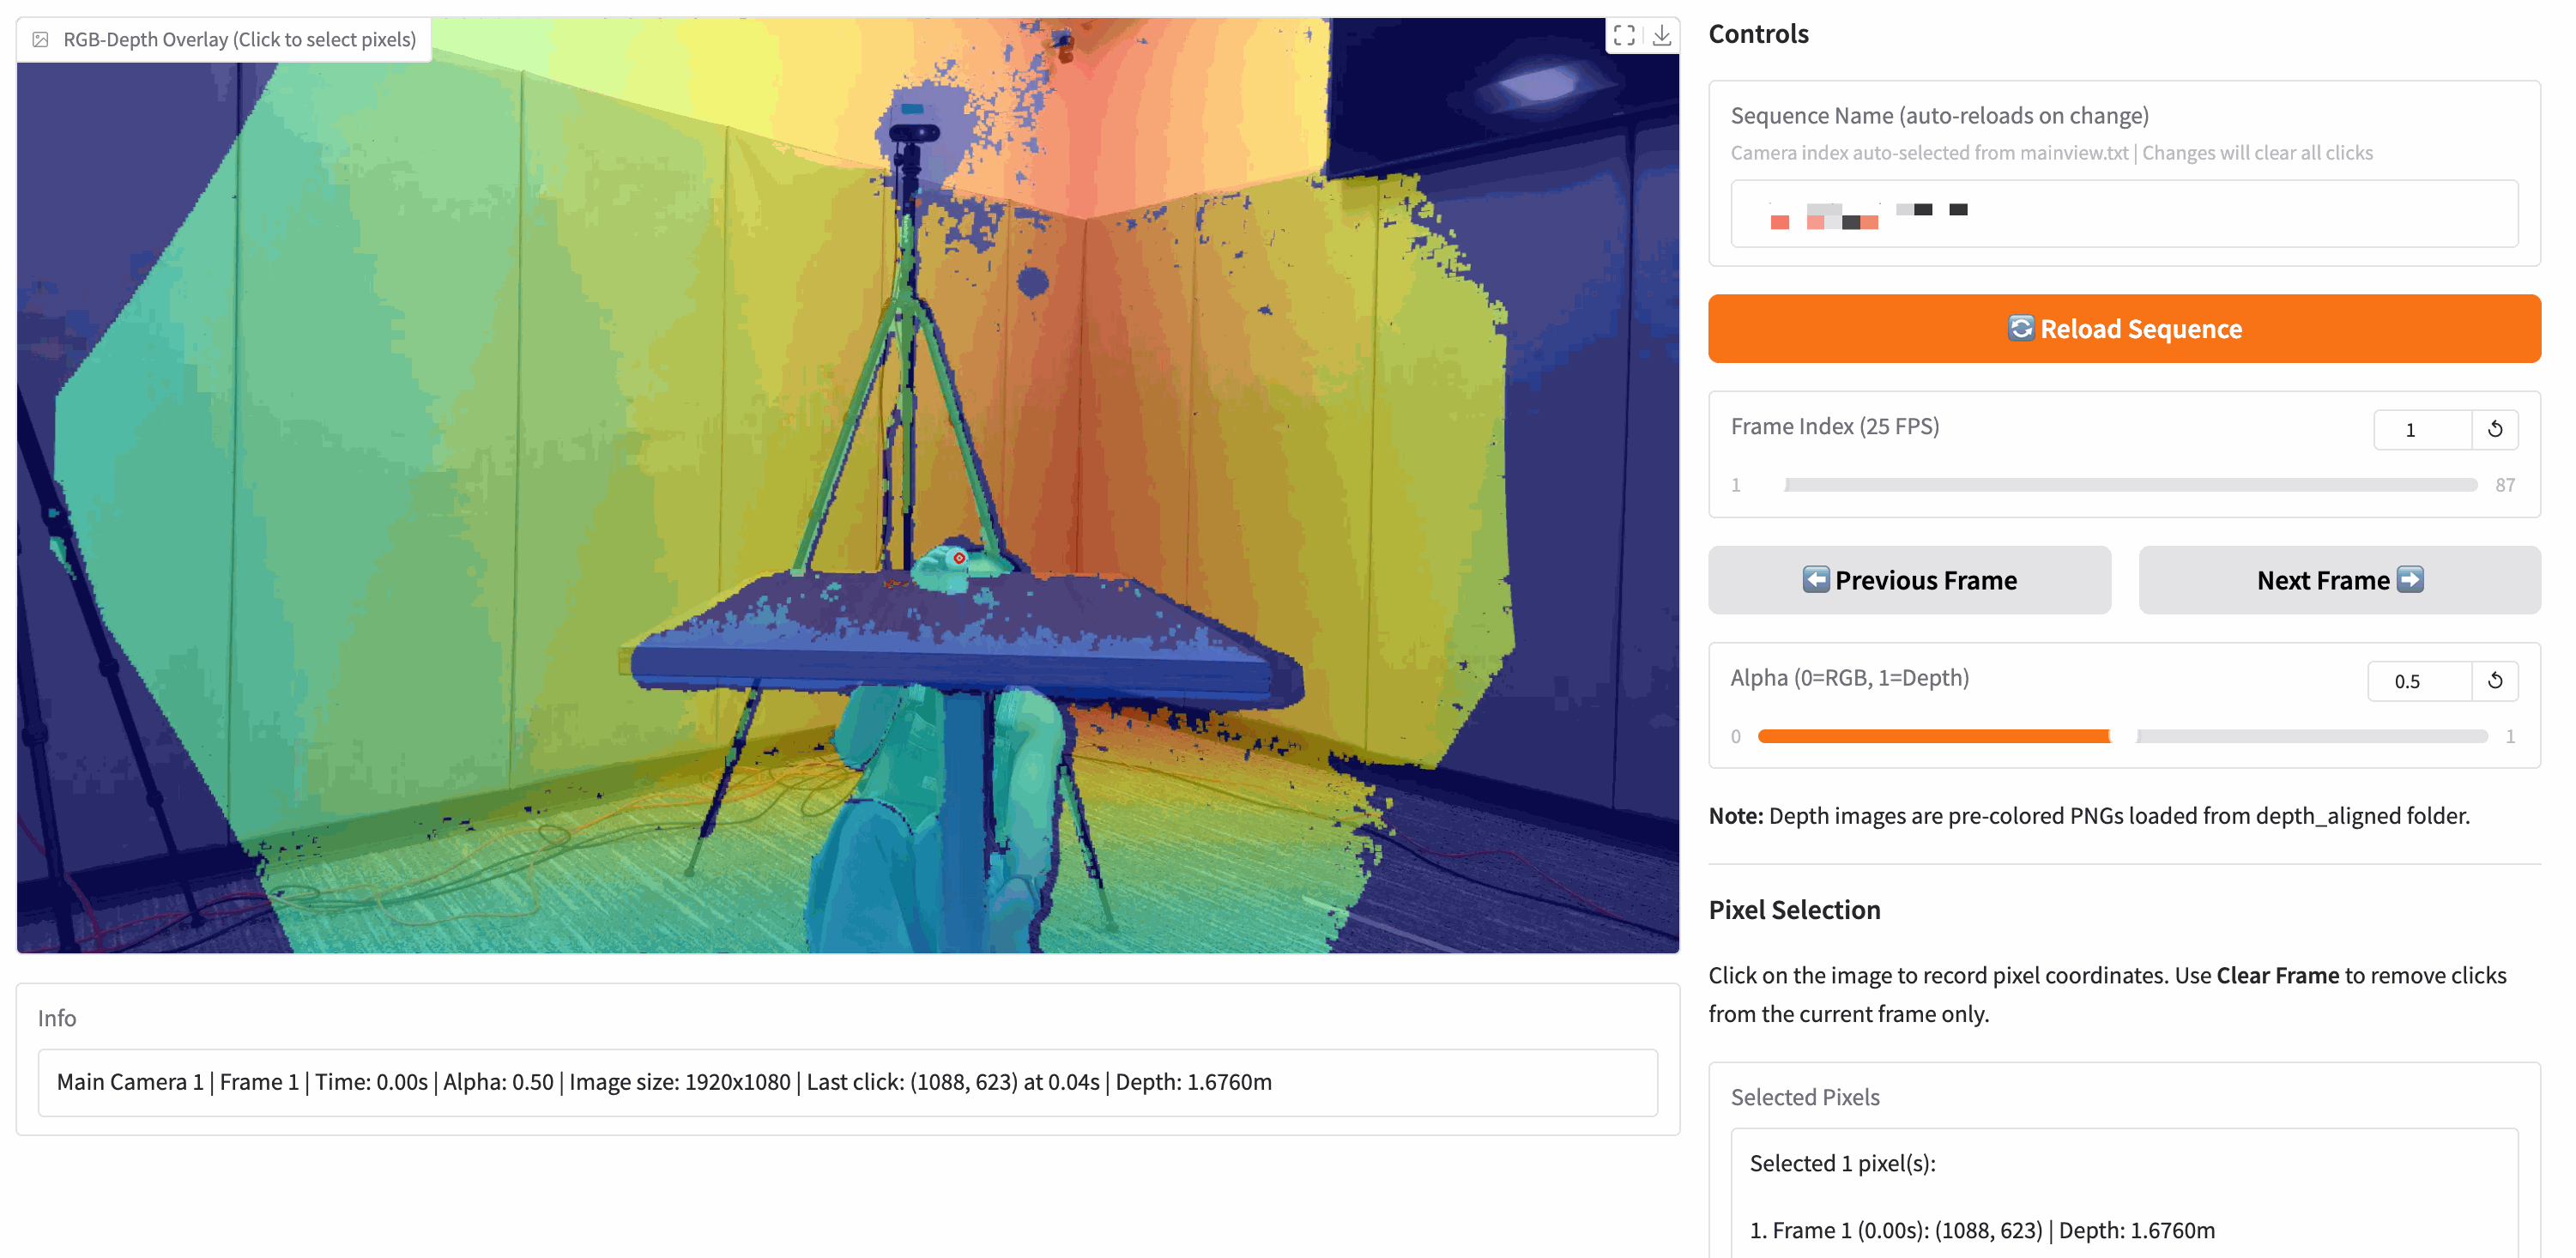
\includegraphics[width=0.99\linewidth]{sec/images/depth_annotator.png}
    \caption{\textbf{The users' interface of the tool we have developed for obtaining depth value.}}
    \label{fig:depth_annotator}
\end{figure*}


\noindent\textbf{List of objects used.} Table~\ref{tab:object-list} lists all physical objects used in our controlled lab videos, together with their measured dimensions.
These objects serve either as priors (with known size) or as inference targets in our kinematic tasks.
All measurements are taken with a ruler or caliper in metric units before filming.


\subsection{Internet Scraping}


\begin{figure}[t]
    \centering
    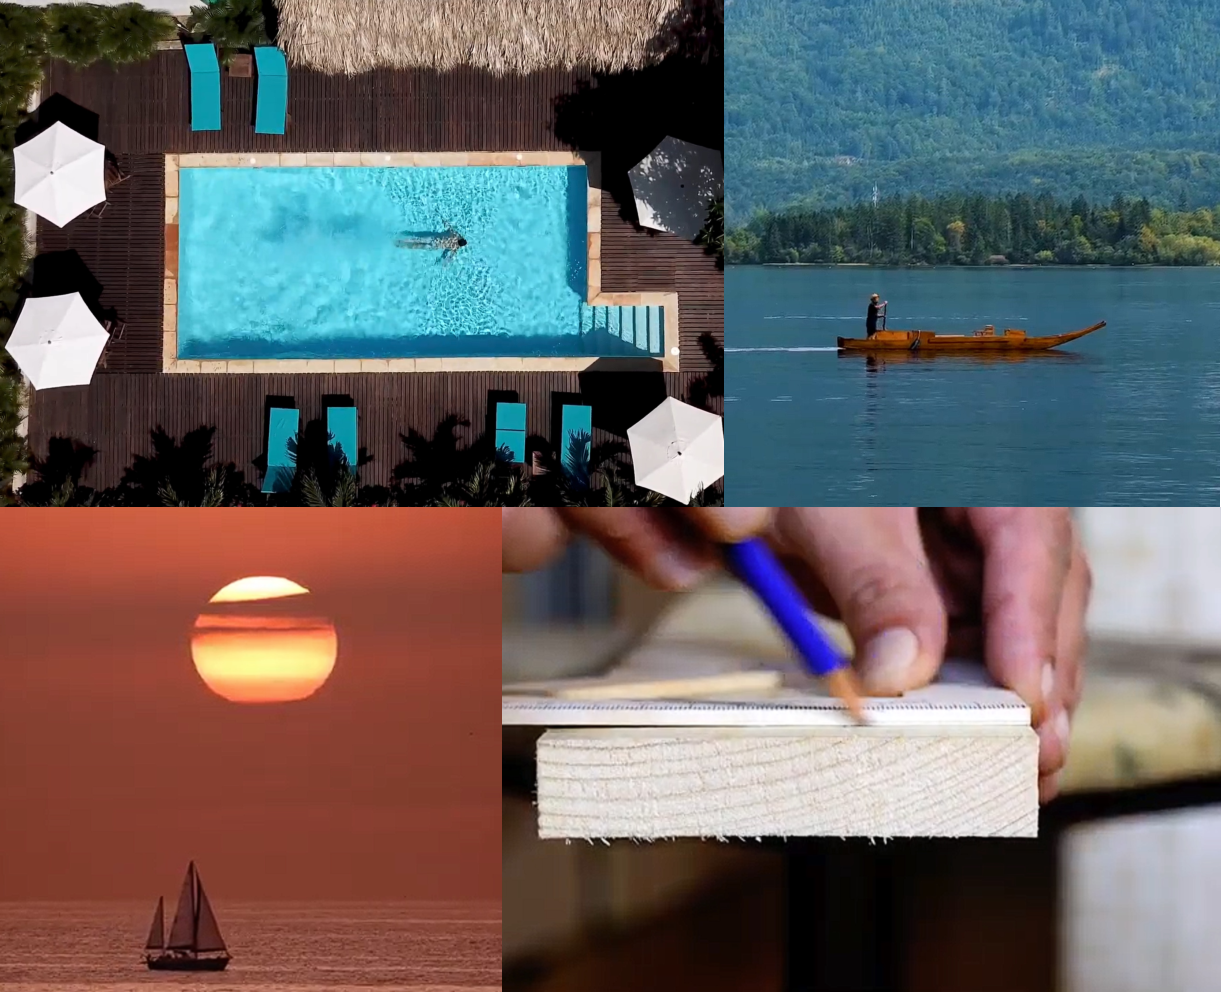
\includegraphics[width=0.99\linewidth]{sec/images/internet_showcase1.pdf}
    % \vspace{-0.5em}
    \caption{\textbf{Examples of videos from open-source platforms.}}
    \label{fig:internet_showcase1}
\end{figure}

\begin{figure}[t]
    \centering
    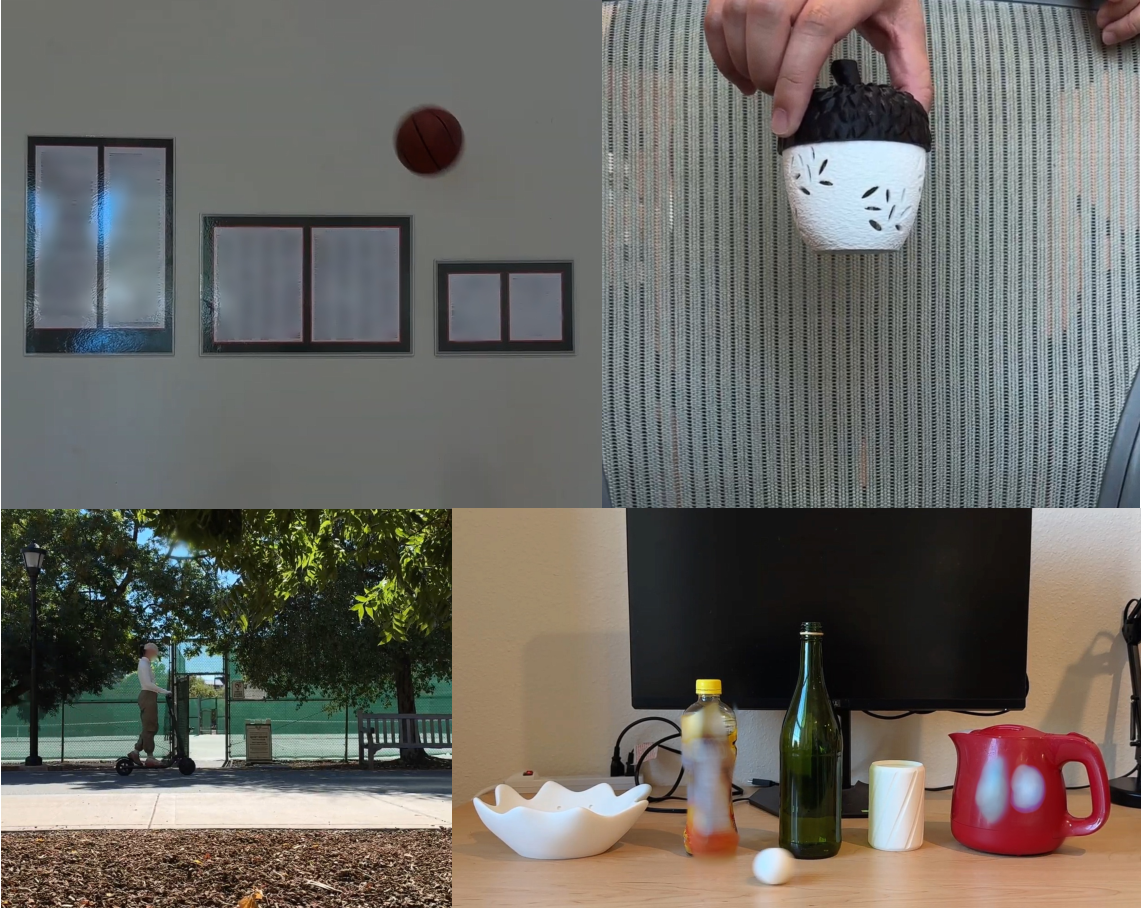
\includegraphics[width=0.99\linewidth]{sec/images/internet_showcase2.pdf}
    % \vspace{-0.5em}
    \caption{\textbf{Examples of self-recorded videos with identity removed.}}
    \label{fig:internet_showcase2}
\end{figure}

Our ``internet'' split in \textsc{QuantiPhy} consists of real-world videos captured by commodity cameras, and is constructed from two sources that we treat under a unified category:
(i) open-source online video platforms, contributing 42 clips;
and (ii) videos recorded by the authors using smartphone rear cameras in everyday indoor and outdoor environments, contributing 30 clips.
All of these videos are direct camera recordings of natural scenes, and thus closely reflect the statistics and imperfections of the physical world.

\noindent\textbf{Why only 2D inference from internet data.}
Unlike our simulation and controlled-lab settings, internet videos do not come with calibrated depth, camera intrinsics, or precise object geometry.
In particular, reliable metric depth is almost impossible to obtain for arbitrary internet footage.
For this reason, we restrict internet videos to 2D kinematic inference tasks.
For each selected clip, we manually construct a pixel ruler, measure pixel-level size/position trajectories of the objects of interest, and then use an approximate scale factor---derived from obvious real-world references in the scene (e.g., gravity $g = 9.8\ \text{m/s}^2$, the length of a credit card, lane width on a road, or the speed of an airport conveyor belt)---to convert these pixel measurements into world-space kinematic quantities.
While this procedure yields reasonably accurate ground truth, it is inherently less precise than the annotation pipelines used for our simulation and lab data.
Consequently, we intentionally keep the proportion of internet data moderate in the overall benchmark.

\noindent\textbf{Videos from open-source platforms.}
We choose open-source video platforms primarily because they avoid copyright issues, offer relatively high image quality, and provide diverse content.
However, videos that satisfy the three screening criteria in \autoref{sec:general_principles} (static camera, at least one rigid object undergoing translational motion, and planar motion for 2D tasks) are relatively rare.
Beyond these core constraints, we additionally require that each candidate clip contain at least one visually obvious physical prior that can be reasonably assumed or measured (e.g., gravity, a credit-card-sized object, standard lane width, or known conveyor-belt speed).
These additional constraints further narrow the pool of usable videos.
There is currently no off-the-shelf automatic pipeline for this selection process, so all internet clips are hand-picked by project members, who visually inspect candidates for compliance with our physical and annotation requirements.
Representative examples are shown in Figure~\ref{fig:internet_showcase1}.

\noindent\textbf{Author-recorded videos.}
Because suitable clips on open-source platforms are scarce, we complement them with 30 videos recorded by the authors using smartphone rear cameras in a variety of everyday scenes, including parking lots, road traffic, bedrooms, and indoor/outdoor sports venues.
During recording, we enforce a fixed camera viewpoint and ensure that at least one rigid object exhibits predominantly translational motion, so that the criteria in \autoref{sec:general_principles} are satisfied.
In many such settings, precise physical quantities (e.g., vehicle speed, basket height) cannot be directly measured.
We therefore annotate these videos using the same pixel-ruler and approximate-scale procedure as for online platform videos, again restricting them to 2D inference tasks.
Example frames from these author-recorded clips are shown in Figure~\ref{fig:internet_showcase2}.


\noindent\textbf{Privacy and anonymization.}
For all internet videos, whether sourced from open platforms or recorded by the authors, we manually inspect frames for sensitive personal information.
Whenever faces, license plates, or other identifying details appear, we apply blurring or masking before including the clip in the dataset.
This ensures that our internet data respect both copyright and privacy constraints while still providing realistic real-world scenarios for quantitative kinematic inference.

\begin{figure*}[t]
    \centering
    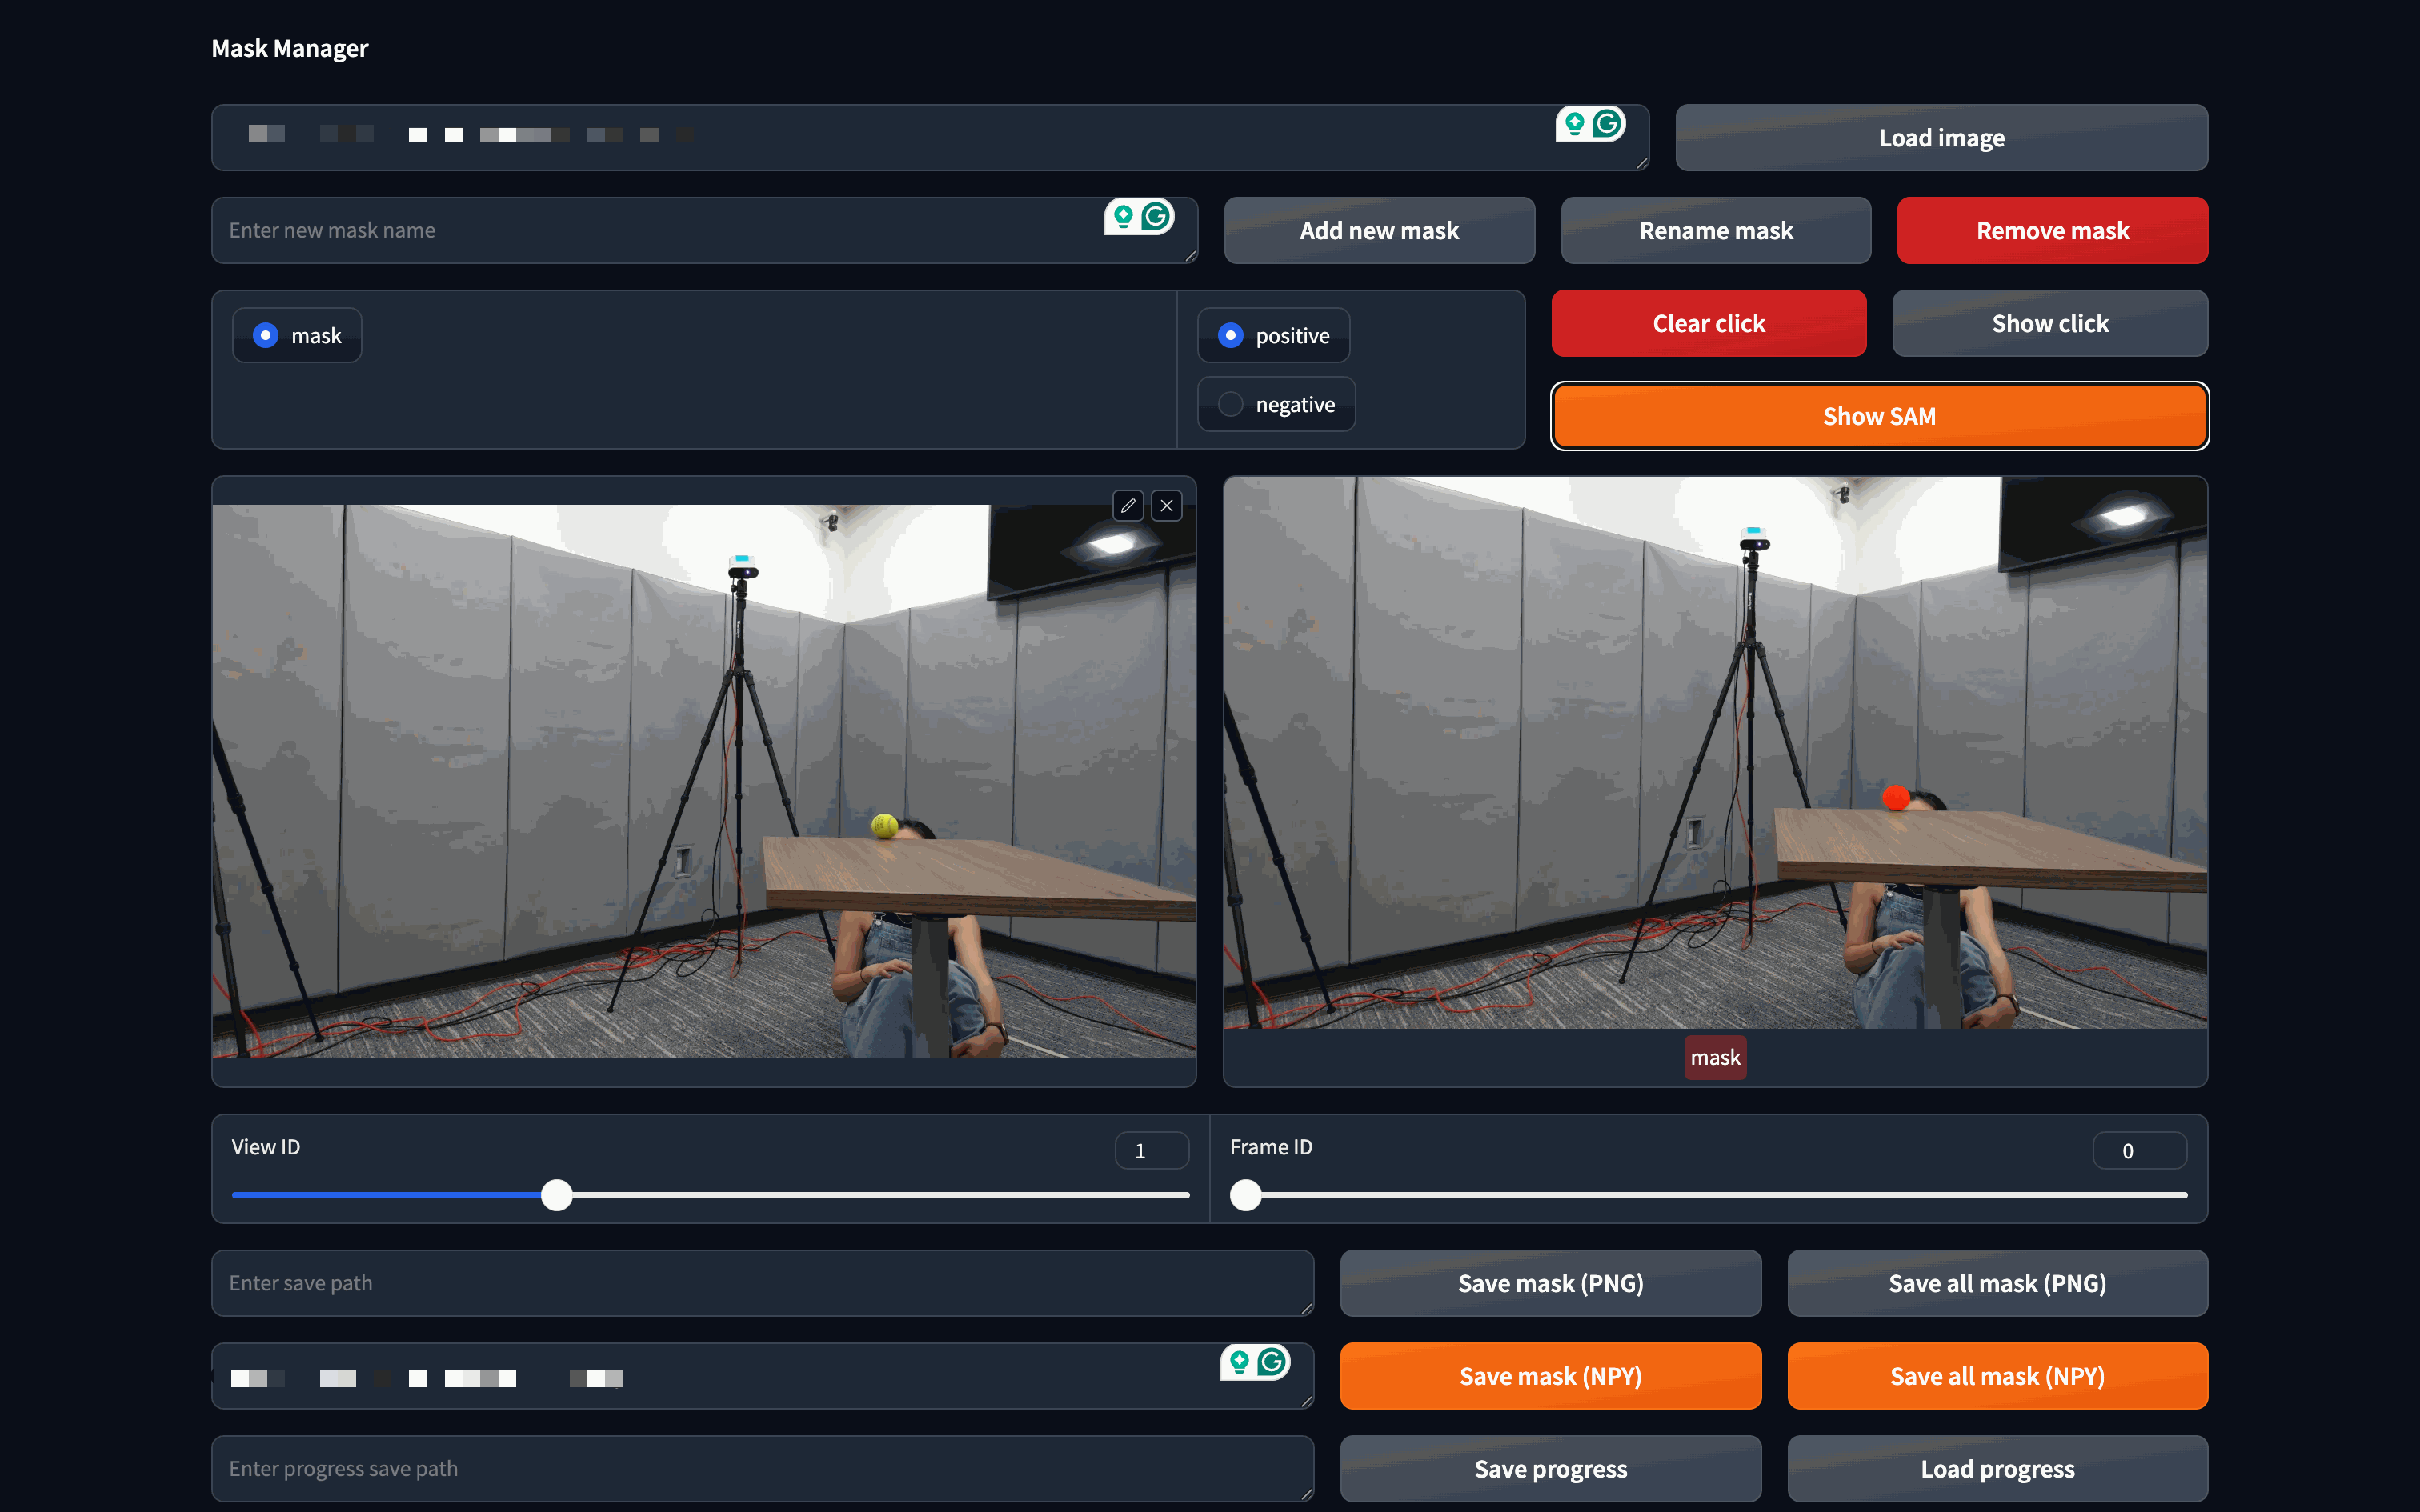
\includegraphics[width=0.99\linewidth]{sec/images/segmentation_ui.png}
    \caption{\textbf{The users' interface of the segmentation tool we have developed.}}
    \label{fig:segmentation_ui}
\end{figure*}


\subsection{Segmented Data}

In \textsc{QuantiPhy}, we aim to benchmark the capabilities of VLMs on videos with diverse background types. Video backgrounds often contain contextual information that may either aid or hinder the inference of a target object's physical properties. To comprehensively study this impact, we design experiments that isolate the target object by completely removing the background. Specifically, we compare the original videos against processed versions where the background has been completely denoised and removed using a segmentation model.

State-of-the-art semantic segmentation models, such as SAM 2~\cite{ravi2024sam2}, have demonstrated robust capabilities in tracking and segmenting arbitrary targets across various tasks. In our experiments, we employ SAM 2 as the backbone segmenter, utilizing a hybrid prompting strategy. To automate the pipeline, we leverage Grounding DINO 1.5~\cite{ren2024grounding} to localize target objects using textual descriptions derived from our video-question pairs. The bounding boxes generated by Grounding DINO serve as box prompts for SAM 2, enabling automatic segmentation.

For complex scenes with multiple objects where the automated pipeline may fail, we incorporate manual intervention by providing point-based prompts to SAM 2. To streamline this workflow, we developed a custom UI-based tool that allows multiple annotators to label objects efficiently, thereby scaling the segmentation process. \autoref{fig:segmentation_ui} illustrates the user interface of this tool, and \autoref{fig:segmented_blender}, \autoref{fig:segmented_lab}, \autoref{fig:segmented_internet} provides exemplary frames of the segmented videos for reference.

\subsection{Quality Control}

The data collection process for \textsc{QuantiPhy} is highly diverse and complex. Since the data originates from heterogeneous sources with varying characteristics, establishing a universal automated protocol for quality assurance is challenging. To address this, we incorporated an additional manual review stage for all candidate data.

To maximize data quality, we manually excluded videos exhibiting excessive motion blur, severe occlusion of the target object, or objects that are difficult to model. Furthermore, we removed videos containing identifiable human subjects to ensure ethical compliance.

Following this review process, approximately 3\% of the Blender data and 30\% of the lab data were discarded, while for the videos scraped from the internet only 72 clips were retained.

\subsection{Ethical Considerations}
In compiling the \textsc{QuantiPhy} dataset, comprising both simulated Blender environments and web-sourced videos, we strictly adhere to all relevant copyright and licensing regulations. For specific data assets requiring attribution, we provide full acknowledgments in the supplementary materials.

We implemented strict privacy measures throughout the data collection and annotation phases to ensure that no personally identifiable information (PII) is retained in the dataset. Relevant Institutional Review Board (IRB) documentation is available upon request. Furthermore, \textsc{QuantiPhy} complies with ethical guidelines regarding content safety; we have rigorously screened the data to exclude biased or harmful content while prioritizing diversity to foster fairness and inclusivity.

\begin{figure*}[ht!]
    \centering
    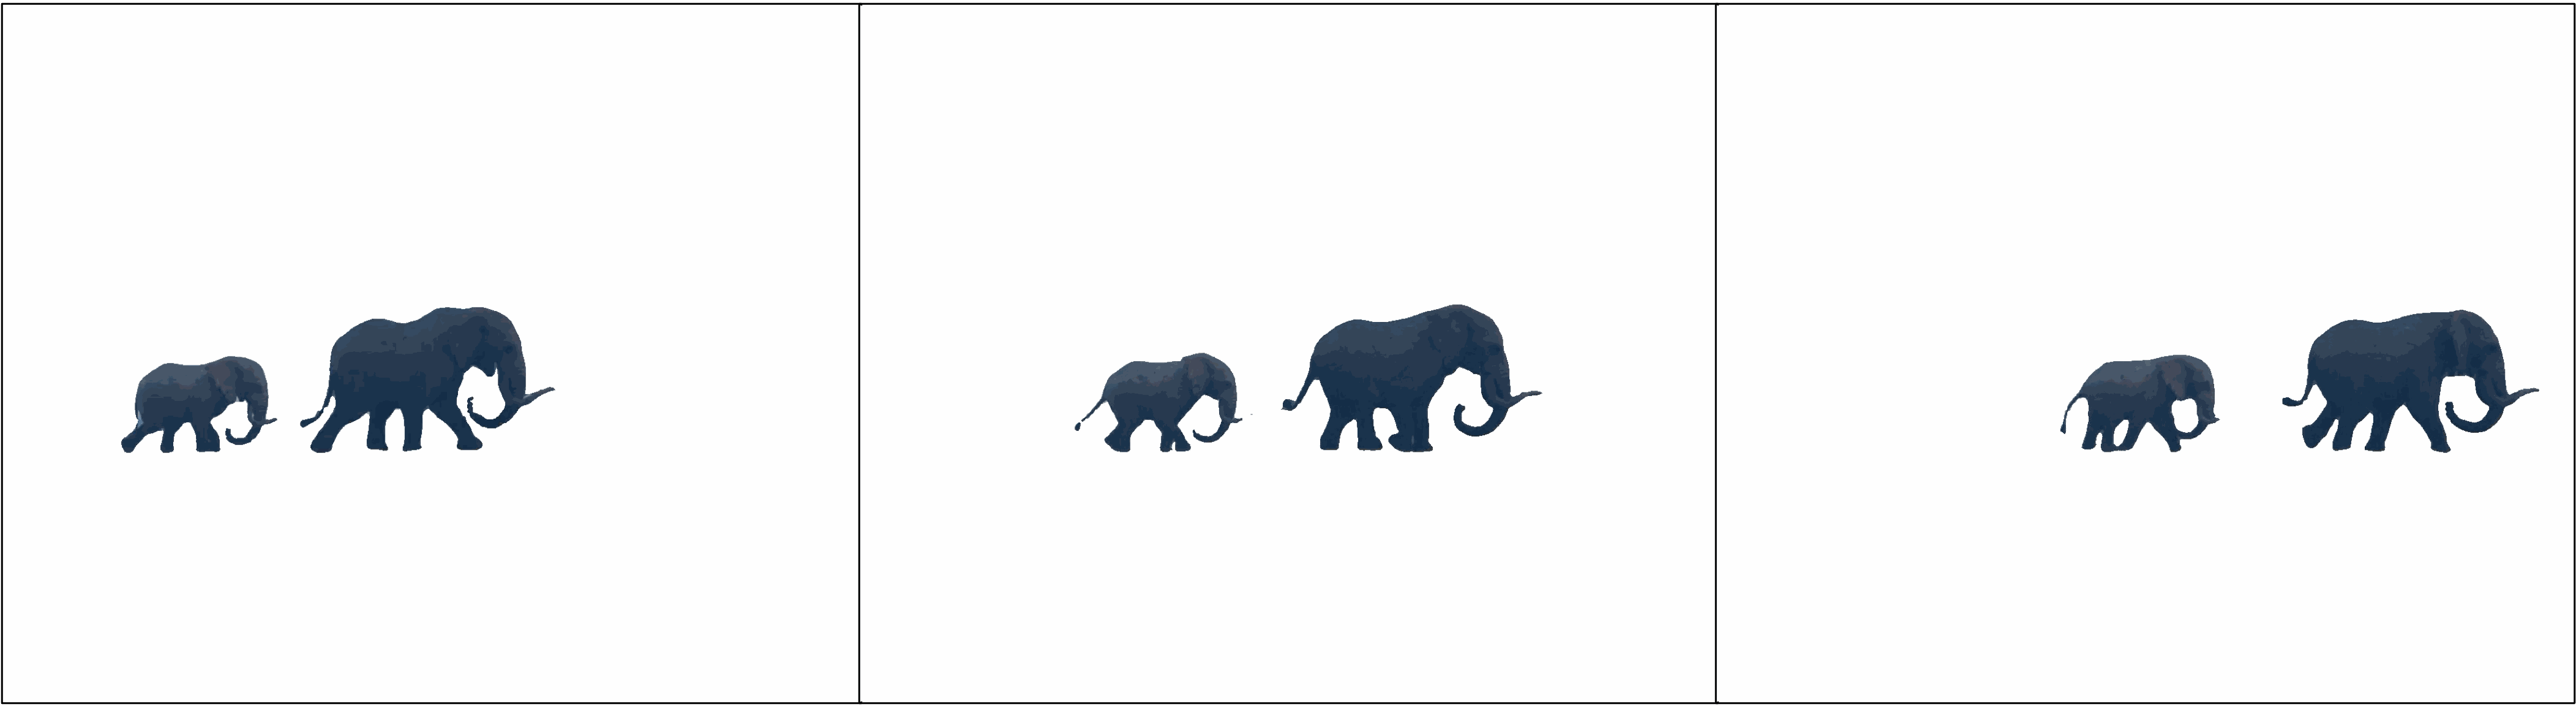
\includegraphics[width=0.99\linewidth]{sec/images/segmented_blender.png}
    \caption{\textbf{Examples of segmented blender data.} After segmentation, we can replace the background image freely.}
    \label{fig:segmented_blender}
\end{figure*}

\begin{figure*}[ht!]
    \centering
    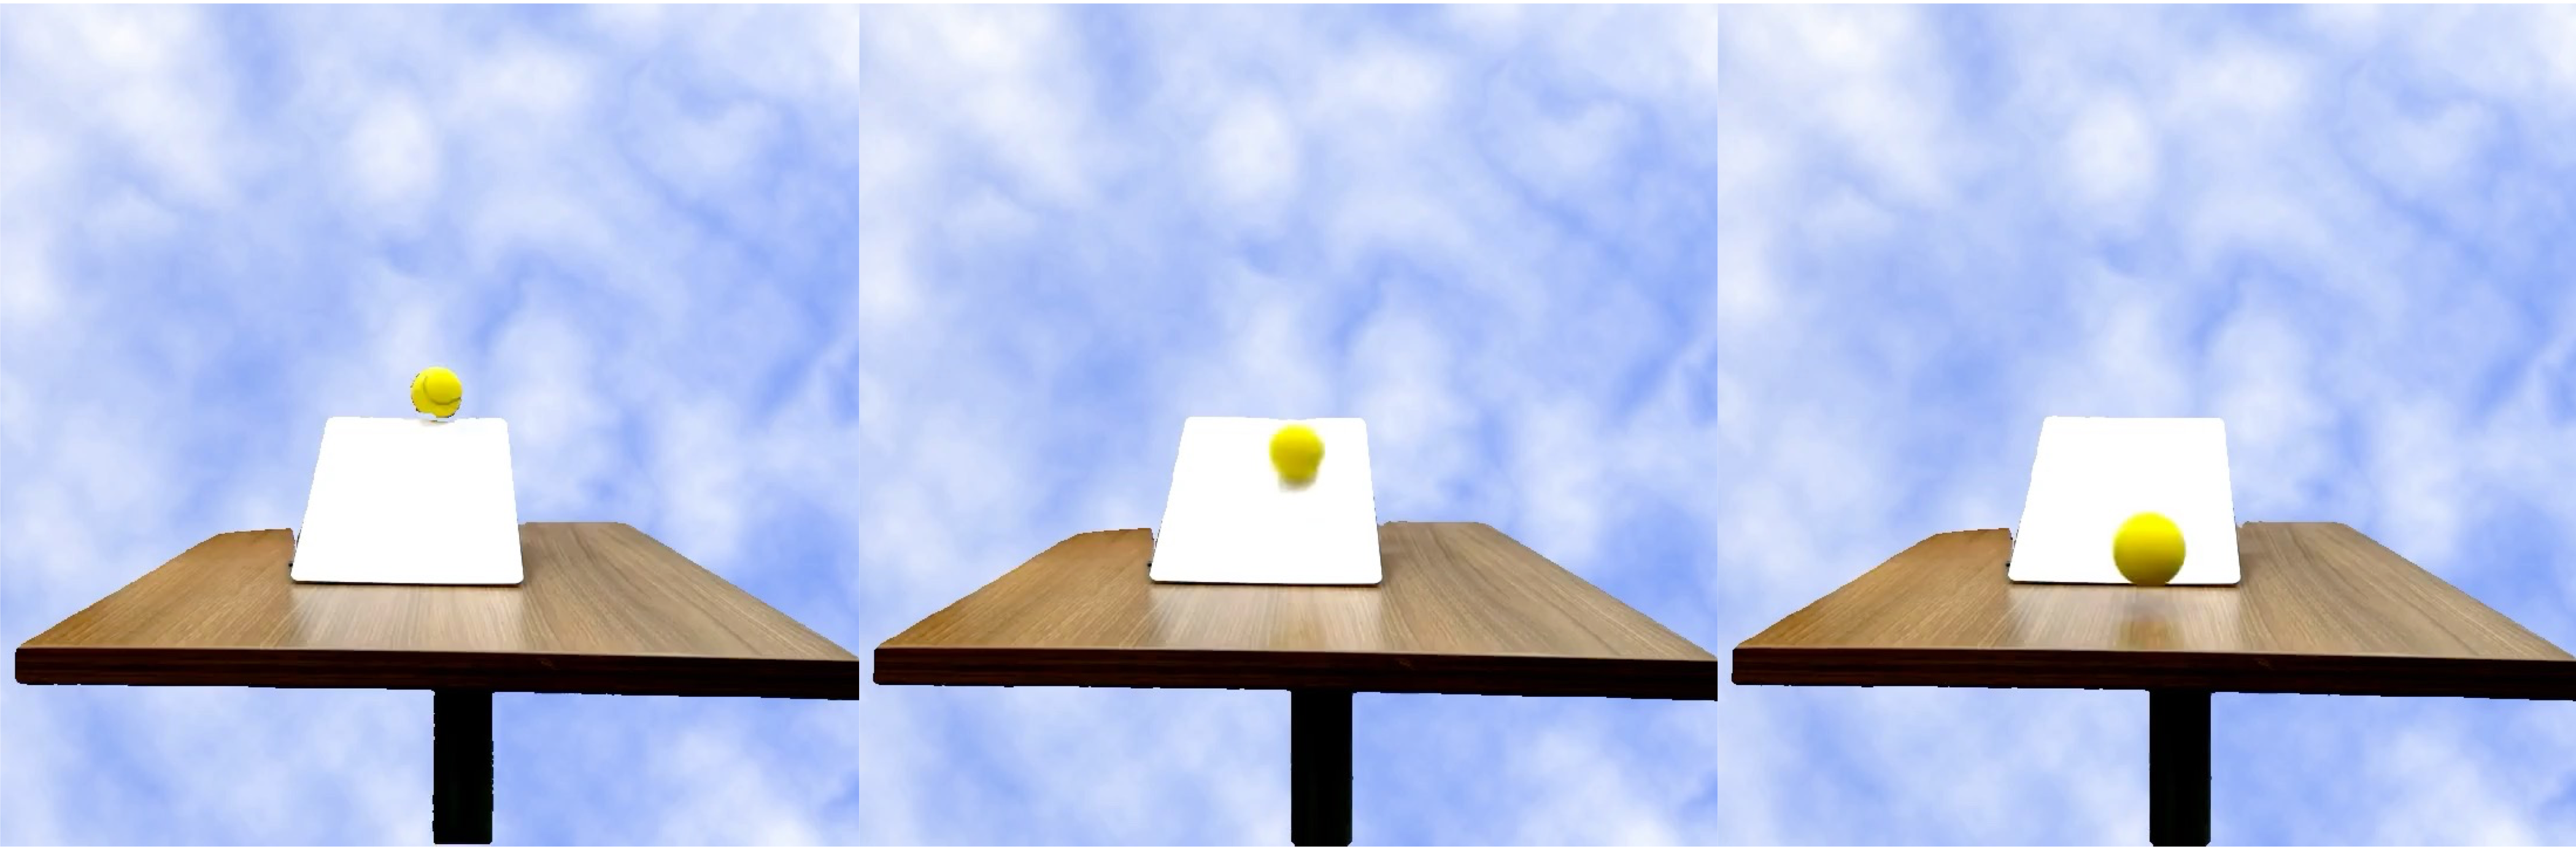
\includegraphics[width=0.99\linewidth]{sec/images/segmented_lab.png}
    \caption{\textbf{Examples of segmented lab data.} After segmentation, we can replace the background image freely.}
    \label{fig:segmented_lab}
\end{figure*}

\begin{figure*}[ht!]
    \centering
    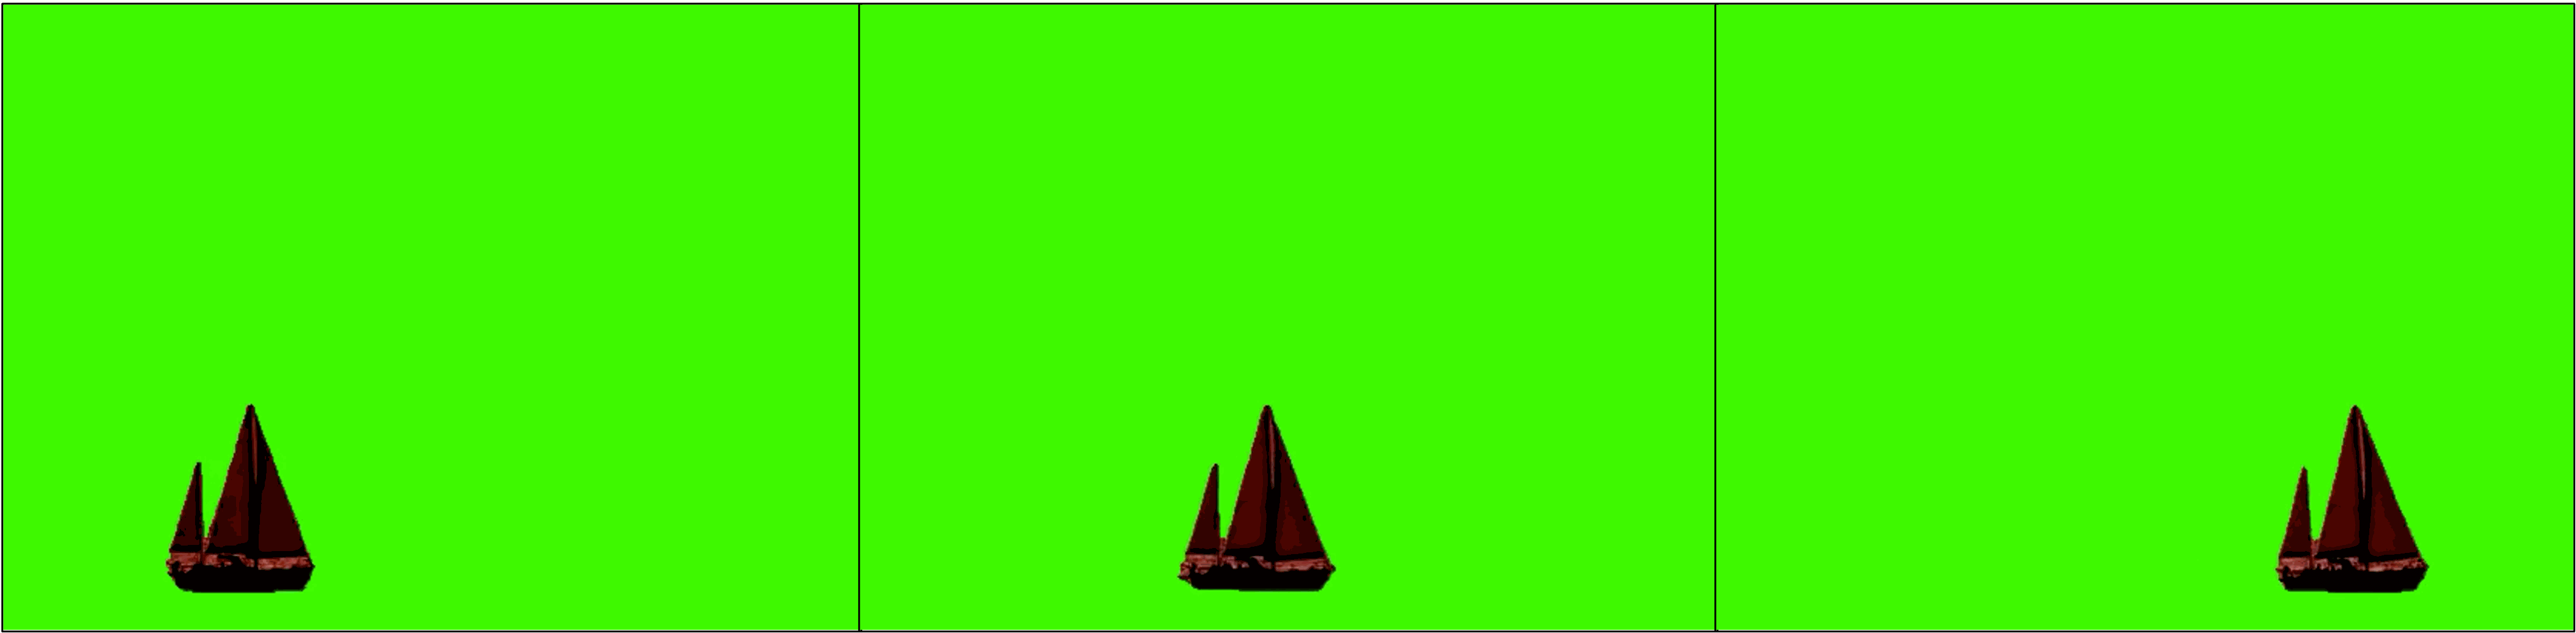
\includegraphics[width=0.99\linewidth]{sec/images/segmented_internet.png}
    \caption{\textbf{Examples of segmented internet data.} After segmentation, we can replace the background image freely.}
    \label{fig:segmented_internet}
\end{figure*}
